%\documentclass[11pt]{beamer}
\documentclass[xcolor=pdftex,dvipsnames,table]{beamer}


\usepackage[utf8]{inputenc}
\usepackage[spanish]{babel}
\usepackage{amsmath}
\usepackage{amsfonts}
\usepackage{amssymb}
\usepackage{graphicx}
\usepackage{lipsum}
\usepackage{ragged2e}
\usepackage{hyperref}
\usepackage{float}
\usepackage{url}
%\usetheme{Frankfurt}
\useinnertheme[shadow]{rounded}
\usepackage{comment}

\usepackage{svg}
\usepackage{tcolorbox}
\usepackage{xcolor}
\usepackage[absolute,overlay]{textpos}
\usepackage{caption}
\usepackage{subcaption}
\usepackage{booktabs}
\usepackage{colortbl}

%%%%%%%%%%%%%%%%%%%%%%%%%%%%%%%%%%%%%%%%%%%%%%%%%%%%%%%%%%%%%%%%%%%%%%%%%%%%%%%!
%%%%%%%%%%%%%%%%%%%%%%%%%%%%  B E G I N   F I L E  %%%%%%%%%%%%%%%%%%%%%%%%%%%%!
%%%%%%%%%%%%%%%%%%%%%%%%%%%%%%%%%%%%%%%%%%%%%%%%%%%%%%%%%%%%%%%%%%%%%%%%%%%%%%%!


%% USACH Corporative Colors

% NEW COLORS 2016 // Primarios
%\definecolor{OrangeUsach}{RGB}{234,118,0}
%\definecolor{GrayUsach}{RGB}{177,177,177}
%\definecolor{BlueUsach}{RGB}{0,47,108}

% NEW COLORS 2016 // Secundarios
\definecolor{OrangeUsach}{RGB}{163,31,52}
\definecolor{GrayUsach}{RGB}{57,64,73}
\definecolor{BlueUsach}{RGB}{138,139,140}


%\definecolor{OrangeUsach}{RGB}{231,91,43}
%\definecolor{BlueUsach}{RGB}{8,60,135}
%\definecolor{GrayUsach}{RGB}{57,64,73}
%\definecolor{GrayUsach}{RGB}{230,230,230}
%\definecolor{GrayUsach}{gray}{0.4}


%% ROBOTO FONT
%\usepackage[sfdefault,thin]{roboto}
\usepackage[sfdefault,light,condensed]{roboto}
\usepackage[T1]{fontenc}

\usefonttheme[onlymath]{serif}
\renewcommand\mathfamilydefault{\rmdefault}


\mode<presentation>{
\usetheme{Rochester}
\setbeamersize{text margin left=4mm,text margin right=4mm}
\setbeamertemplate{navigation symbols}{}

\usecolortheme[named=BlueUsach]{structure}
\setbeamercovered{transparent}
%%%
\setbeamercolor{background canvas}{bg=BlueUsach, fg=white}
\setbeamercolor{title}{fg=red}
%
%\setbeamercolor{secsubsec}{fg=white,bg=black}
\setbeamercolor{normal text}{fg=white}
%%
\setbeamercolor{alerted text}{fg=OrangeUsach}
%\setbeamercolor{figures}{fg=white,bg=black}
%
\

\setbeamercolor{frametitle}{fg=GrayUsach}
\setbeamercolor{framesubtitle}{fg=GrayUsach}
%
%\setbeamerfont{frametitle}{series=\bfseries}
%\setbeamercolor{frametitle}{fg=white}

%\setbeamerfont{framesubtitle}{size=\large}
%\setbeamercolor{framesubtitle}{fg=OrangeUsach}
%
\setbeamercolor{section in toc shaded}{fg=GrayUsach}
\setbeamercolor{section in toc}{fg=GrayUsach}
%
\setbeamercolor{item projected}{bg=OrangeUsach}
\setbeamercolor*{enumerate item}{fg=GrayUsach}
\setbeamercolor*{enumerate subitem}{fg=GrayUsach}
\setbeamercolor*{enumerate subsubitem}{fg=GrayUsach}
%
\setbeamercolor*{itemize item}{fg=OrangeUsach}
%
\setbeamercolor*{description item}{fg=OrangeUsach}
%
%
%% Setting for Black and White
\setbeamercolor{section in head/foot}{bg=white, fg=black} % BW
\setbeamercolor{background canvas}{bg=white, fg=black} % BW
\setbeamercolor{normal text}{fg=black} % BW
\setbeamercolor{title}{fg=white,bg=BlueUsach!70!white} % BW
%\setbeamercolor{title}{fg=black,bg=NavyBlue!10!white}



\setbeamercolor{section in toc}{fg=black} % BW
\setbeamercolor{frametitle}{fg=black,bg=white} % BW
\setbeamercolor{framesubtitle}{fg=GrayUsach}
\setbeamercolor{section in toc shaded}{fg=black} % BW
}


%
\usepackage[spanish]{babel}
\usepackage[utf8]{inputenc}




\usepackage{multimedia}
\usepackage{beamerseminar}

\usepackage[absolute,overlay]{textpos}
\usepackage{setspace}
\usepackage{comment}
\usepackage{moreverb}
\usepackage{graphicx}
\usepackage{hyperref}
\usepackage{amsmath,wasysym}
\usepackage{amsfonts,bm}
\usepackage[mathscr]{eucal}
\usepackage{mathrsfs}
%\usepackage{cclicenses}
\usepackage[scale=1.2]{ccicons}
\usepackage{multimedia}
%\usepackage{media9}
%\usepackage[framemethod=TikZ]{mdframed}
%
\usepackage{tikz,pgfplots}
\usetikzlibrary{calc}
\usetikzlibrary{intersections}
\usetikzlibrary{arrows, patterns}
\usetikzlibrary{decorations.pathmorphing}
\usetikzlibrary{decorations.markings}
\usetikzlibrary{positioning}
\usepgflibrary{shapes.geometric}
%\usetikzlibrary{trees}
%\usetikzlibrary{3d}

%\usetikzlibrary{shadows}

%\usetikzlibrary{pgfplots.units}
%\usepgfmodule{plot}
%\pgfplotsset{width=8cm}
%\pgfplotsset{compat=1.3,compat/path replacement=1.5.1}
%
%
%\usetikzlibrary{external}
%\tikzexternalize
%\tikzset{external/export=true}
%\tikzsetexternalprefix{../External/}
%
%\usepackage{beamerthemesplit}
%\usepackage[showboxes]{textpos}
%\usepackage{xmpmulti}
%\usepackage{colortbl}
%\usepackage{beamertexpower}
\renewcommand{\bfdefault}{sbc}
%
%
\newcommand{\Codigo}{}
\newcommand{\Titulo}{}
\newcommand{\SubTitulo}{}
\newcommand{\Autor}{}
\newcommand{\Correo}{}
\newcommand{\Fecha}{}
\newcommand{\Correooo}{}
\newcommand{\LastUpdate}{}

%------------------------------------------------------------------------------!
% Settings for package: HyperRef **********************************************!
%
\hypersetup{
pdfpagemode=FullScreen,
baseurl={roberto.ortega@usach.cl},
pdftitle={Presentación Programa de Magister},
pdfauthor={Roberto Ortega},
pdfcreator={Roberto Ortega},
pdfproducer=PDFLaTeX,
pdfsubject={Presentación Programa de Magister},
pdfkeywords={}
}
%
%
%------------------------------------------------------------------------------!
% New commands ****************************************************************!
%
\newcommand{\orange}{\textcolor{OrangeUsach}}
\newcommand{\gray}{\textcolor{GrayUsach}}
\newcommand{\blue}{\textcolor{BlueUsach}}

\newcommand{\white}{\textcolor{white}}
\newcommand{\green}{\textcolor{green}}
\newcommand{\yellow}{\textcolor{yellow}}
\newcommand{\red}{\textcolor{red}}
\newcommand{\violet}{\textcolor{violet}}
\newcommand{\cyan}{\textcolor{cyan}}
\newcommand{\black}{\textcolor{black}}



\newcommand{\TitleFrame}{}
\newcommand{\SubTitleFrame}{}
%
%------------------------------------------------------------------------------!
% Settings for beamer style ***************************************************!
% 
%% Formato de las secciones en la tabla de contenidos
%
%% Menu interactivo
%% Al comienzo de cada \section
%\AtBeginSection{%
%\begin{frame}[t]
%%\frametitle{Indice}
%\tableofcontents[currentsection]
%\end{frame}}
%%% Al comienzo de cada \subsection
%\AtBeginSubsection{%
%\begin{frame}[t]
%%\frametitle{Indice}
%\tableofcontents[currentsection,currentsubsection]
%\end{frame}}
%
%

%% Formato pie de página
\setbeamertemplate{footline}{%
\begin{beamercolorbox}{section in head/foot}
\vskip3pt%
\makebox[0.90\textwidth][l]{%
\hspace{2mm}\href{mailto:\Correo}{\sf \Correo}
\hspace{1mm}\orange{\ccLogo\:\ccAttribution}
\hspace{1mm}\gray{\Titulo}
$\:|\:$\orange{\SubTitulo}
}%
%%\ccLogo$\quad$\ccAttribution$\:$\ccNonCommercial$\:$\ccNoDerivatives\\
\makebox[0.10\textwidth][c]{%
{\sf \insertframenumber\;of\;\inserttotalframenumber}}
\vskip2pt
\end{beamercolorbox}
% 
% LAST UPDATE
\begin{tikzpicture}[remember picture,overlay]
\node[gray,above right,rotate=90, scale=0.7, xshift=1mm] at (current page.south east)
{\em\tiny \orange{$\circledast\:$}\LastUpdate\orange{$\:\circledast$}};
\end{tikzpicture}%
}


\addtobeamertemplate{frametitle}{}{%
\begin{tikzpicture}[remember picture,overlay]

%% NUEVO LOGO
\node[below left=1mm] at (current page.north east)
{
\includegraphics[height=1cm]{USACH2016_RIGHT_BW}};
	
%% ORANGE & BLUE RECTANGLES
\draw[draw=BlueUsach,fill=BlueUsach] (current page.north east) rectangle ([yshift=-1.5mm]current page.north);
\draw[draw=OrangeUsach,fill=OrangeUsach] (current page.north west) rectangle ([yshift=-1.5mm,xshift=3.5cm]current page.north);

%\node[below left] at (current page.north east)
%	{\includegraphics[height=1cm]{/Users/Roberto/Dropbox/Documents/USaCh/Corporativo/SetHorAi/UDS_HCOLOR}};

%\node[below left] at (current page.north east)
%	{\includegraphics[height=1cm]{/Users/Roberto/Dropbox/Documents/USaCh/Corporativo/SetHorAi/UDS_HBCO}};

\end{tikzpicture}
\vspace{-10mm}}
%
%% Incluye únicamente las etiquetadas como {label=ok}
%\includeonlyframes{index,ok}
%
%
%

\newcommand{\Cover}{%
\begin{tikzpicture}[remember picture,overlay, opacity=1]
%
\node[below,yshift=-10mm] at (current page.north)
	{
\includegraphics[width=7cm]{Logos/mit.png}};
%

%% ORANGE & BLUE RECTANGLES
\draw[draw=OrangeUsach,fill=OrangeUsach] (current page.north west) rectangle ([yshift=-3mm]current page.north);
\draw[draw=BlueUsach,fill=BlueUsach] (current page.north east) rectangle ([yshift=-3mm]current page.north);


\node[below, align=center, yshift=-5cm] at (current page.north){%
	\orange{\Large\bf \Codigo}\\
	\gray{\large\bf \Titulo}\\
	\orange{\SubTitulo}\\[5mm]
	\gray{\scriptsize\Autor}\\
	%\orange{{\scriptsize\Correo}}\\[3mm]
	\gray{\scriptsize\Fecha}};
%
\end{tikzpicture}}


%%%%%%%%%%%%%%%%%%%%%%%%%%%%%%% E N D   F I L E %%%%%%%%%%%%%%%%%%%%%%%%%%%%%%%!
%%%%%%%%%%%%%%%%%%%%%%%%%%%%%%%%%%%%%%%%%%%%%%%%%%%%%%%%%%%%%%%%%%%%%%%%%%%%%%%!

\newcommand{\celda}[1]{
	\begin{minipage}{2.5cm}
		\vspace{5mm}
		#1
		\vspace{5mm}
	\end{minipage}
}

\usefonttheme[onlymath]{serif}

\renewcommand{\Codigo}{}
\renewcommand{\Titulo}{Proyecto Capstone}

\renewcommand{\Autor}{Elías Ortega M.}
\renewcommand{\Correo}{ivan.fernandez.g@usach.cl}
\renewcommand{\Correooo}{rodrigo.sotoc@usach.cl}


\addtobeamertemplate{frametitle}{}{%
\begin{textblock*}{\textwidth}(.80\textwidth,0.03\textwidth)

\includegraphics[width=0.25\textwidth]{Logos/mit.png}
\end{textblock*}}

\author[ Iván  Fernández G.]{
Autor: Iván Alejandro Fernández Gracia\inst{1} \\
Profesores: John R. Williams\inst{2} & Abel Sanchez\inst{3}  & Carolina Barreiro\inst{4}
}



\title{\color{Black} Certificado Profesional en Programación: Desarrollo Full-Stack con MERN}
\date{22 de abril de 2022} 
%\subtitle{De primer a tercer orden}
%\logo{
\includegraphics[scale=0.0975]{Logos/logo_usach_0.png}}
\institute[USACH]{
	\inst{1}
		Fullstack y Mobile Developer. Ingeniero Civil Mecanico, Universidad de Santiago de Chile.\\
	\inst{2}
		Profesor de Ingeniería de la Información en el Departamento de Ingeniería Civil y Ambiental del MIT.\\
	\inst{3}
		Científico investigador y Director Ejecutivo del Centro de Datos Geoespaciales del MIT.\\
	\inst{4}
		Digital Animation Engineer & Project Management Specialist de la Universidad Panamericana, Mexico.\\
		\vspace{0.5mm}
}





\AtBeginSection[]
{
	\begin{frame}<beamer>{\textbf{Contenido}}
	\small{
		\tableofcontents[currentsection,currentsubsection]
		}
	\end{frame}
}
%%%%%%%%%%%%%%%%%%%%%%%%%%%%%%%%%%%%%%%%%%%%%%%%%%%%%
%%%%%%%%%%%%%%%%%%%%% EMPIEZA %%%%%%%%%%%%%%%%%%%%%%%%%%%%
%%%%%%%%%%%%%%%%%%%%%%%%%%%%%%%%%%%%%%%%%%%%%%%%%%%%%%

\begin{document}
\addtobeamertemplate{block begin}{\setlength\abovedisplayskip{0pt}}

	\begin{frame}

% 		\begin{textblock*}{0.25\textwidth}(0.12\textwidth,0.6\textwidth)
% 		\begin{figure}
% 		    \centering
% 		    
\includegraphics[width=1.0\linewidth]{Logos/scmc.png}
% 		\end{figure}
% 		\end{textblock*}
		\begin{textblock*}{\textwidth}(.8\textwidth,0.05\textwidth)
		%\begin{textblock*}{0.3\textwidth}(0.7\textwidth,0\textwidth)
%		\begin{figure}
%		    \centering
		    
\includegraphics[width=0.25\linewidth]{Logos/mit.png}
%		\end{figure}
		\end{textblock*}
		
		\begin{textblock*}{\textwidth}(-0.01\textwidth,0.03\textwidth)
		    
\includegraphics[width=0.23\linewidth]{Logos/MIT-Simbolo.png}
		\end{textblock*}
		
		
		\begin{textblock*}{\textwidth}(.37\textwidth,0.03\textwidth)
		    
\includegraphics[width=0.30\linewidth]{Logos/mernlogo.jpg}
		\end{textblock*}
		
		\maketitle
		
		
	\end{frame}

	\begin{frame}{\textbf{Contenido}}
	\small{
		\tableofcontents}
	\end{frame}

%------------------------------- [(1)START OBJETIVOS] ----------------------------------------
\section{Introducción y Objetivos}
%------------------------------------------------------------
\begin{frame}{Introducción y Objetivos del Proyecto}
        \justifying
        \small
        \setbeamercolor{block title}{use=structure,fg=white,bg=black!75!black}
        \setbeamercolor{block body}{use=structure,fg=black,bg=black!10!white}		
        \begin{block}{Objetivos}
            \justifying
            \begin{enumerate}
                \justifying
                \item {\textbf{Evaluar} los conocimientos sobre la construcción, testeo y despliegue de una aplicación web \textbf{MERN} stack, \textbf{API} de backend con Express, \textbf{React} , pipeline de integracion continua (Continuous Integration) / entrega continua (Continuous Delivery) \textbf{(CI/CD)}, interaccion con \textbf{base de datos}, \textbf{cybersecurity}  y mucho mas.}
                \item {\textbf{Crear} una  \textbf{aplicación bancaria} donde los usuarios puedan registrarse para realizar  \textbf{retiros, depositos, pagos}, etc.}
            \end{enumerate}
            
        \end{block}	
\end{frame}
%------------------------------- [END OBJETIVOS] ----------------------------------------

%------------------------------- [START Three-Tiered ] ----------------------------------------
\section{Three-Tiered Applications}

%------------------------------------------------------------
\begin{frame}{Diagrama Three-Tiered con Tecnologias}
\small{

    \begin{textblock*}{0.9\textwidth}(0.05\textwidth,0.1\textwidth)
        \setbeamercolor{block title}{use=structure,fg=white,bg=gray!75!}
        \setbeamercolor{block body}{use=structure,fg=black,bg=gray!10!white}
        \begin{block}{Tecnologias y motivo} 
                    \scriptsize  {
                    \justifying
                    \begin{itemize}
                      \setlength\itemsep{0.1em}
                        \item {\textbf{Frontend}: El \textbf{diseño UI/UX} del sitio web es implementado con el framework \textbf{React}.}
                        \item {\textbf{Backend}: El servidor que maneja las \textbf{peticiones de recursos} de los clientes y la \textbf{seguridad de los datos} se implementa con framework \textbf{Express}. Este servidor se conecta con 2 bases de datos.}
                        \item {\textbf{Database}: La base de datos en la nube \textbf{MongoAtlas} se encarga de la persistencia de los datos y \textbf{Redis} del almacenamiento en cache de tokens para la seguridad de la app.}
                    \end{itemize}}
            
        \end{block}
    \end{textblock*}
    
    \begin{textblock*}{0.9\textwidth}(0.05\textwidth,0.38\textwidth)
        \begin{figure}
            \centering
            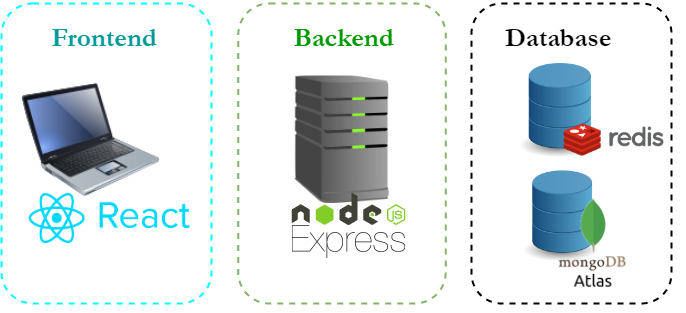
\includegraphics[width=0.8\linewidth]{levels/2leves.png}
            \label{fig:my_label}
        \end{figure}
    \end{textblock*}
    
}
\end{frame}
%------------------------------- [END Three-Tiered ] ----------------------------------------

%------------------------------- [(2) START Arquitectura Frontend ] ----------------------------------------
\section{Arquitectura Frontend}
%------------------------------------------------------------
\begin{frame}{Framework y Estructura de Carpetas}\small{
    \begin{textblock*}{0.56\textwidth}(0.05\textwidth,0.08\textwidth)
            \setbeamercolor{block title}{use=structure,fg=white,bg=cyan!75!}
            \setbeamercolor{block body}{use=structure,fg=black,bg=cyan!10!white}
            \begin{block}{React y Carpetas} 
            \justifying
                Se utiliza \textbf{React} como framework para el frontend de la app. La ilustracion de la derecha muestra la estructura de carpetas. La \textbf{carpeta /scr} contiene subcarpetas que dividen la \textbf{logica} del proyecto con un cierto orden:
                    \vspace{-0.0cm}
                    \footnotesize {
                    \begin{itemize}
                      \setlength\itemsep{0.1em}
                        \item {\textbf{Screens}: Vistas principales o contenedor de muchos componentes.}
                        \item {\textbf{Component}: Componentes que cumplen con una sola funcionalidad.}
                        \item {\textbf{Hooks}: Funciones que te permiten “enganchar” el estado de React y el ciclo de vida desde componentes de función.}
                        \item {\textbf{Routers}: Componentes de navegación}
                        \item {\textbf{Actions, Reducer, store}: Estado de la app REDUX}
                        \item {\textbf{Helpers}: Encapsular funciones utilizadas en muchos componentes}
                    \end{itemize}}
            \end{block}
    \end{textblock*}
    
    
    \begin{textblock*}{0.5\textwidth}(0.6\textwidth,0.075\textwidth)
        \begin{figure}
            \centering
            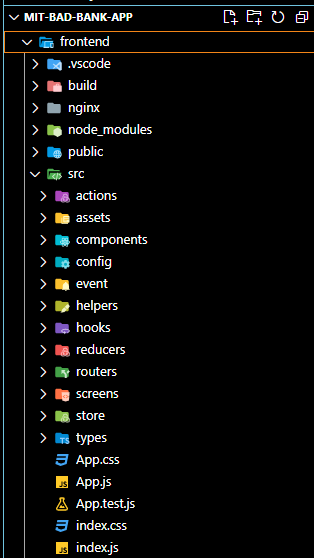
\includegraphics[width=0.75\linewidth]{front/sc2.png}
            % \caption*{Espacio de trabajo robot \\ ABB irb 360-3/800}
            \label{fig:my_label}
        \end{figure}
    \end{textblock*}}
\end{frame}
%------------------------------------------------------------
\begin{frame}{\textbf{Teoría:} Diagrama Componentes React}
    \begin{textblock*}{0.58\textwidth}(0.05\textwidth,0.12\textwidth)
            \setbeamercolor{block title}{use=structure,fg=white,bg=cyan!75!}
            \setbeamercolor{block body}{use=structure,fg=black,bg=cyan!10!white}
            \begin{block}{Definición} 
            \justifying
                Con el fin de explicar mejor la creacion UI y la estructura de la app, se les asigna definiciones a cada componente en React.
                    \vspace{-0.0cm}
                    \begin{itemize}
                        \item {\textbf{State App}: guardan el estado de uno o mas componente}
                        \item { \textbf{Router}: permiten que rutas renderizen otros componente.}
                        \item {\textbf{Screen}: componentes se utilizan como containers de otros conponentes de bajo nivel.}
                        \item {\textbf{Component}: componentes de bajo nivel y/o que desarrollan funcionalidades especificas.}                        
                    \end{itemize}
            \end{block}
    \end{textblock*}
    
    
    \begin{textblock*}{0.5\textwidth}(0.6\textwidth,0.15\textwidth)
        \begin{figure}
            \centering
            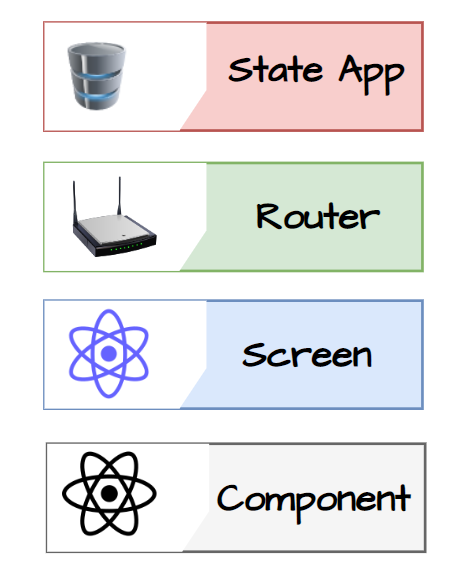
\includegraphics[width=0.75\linewidth]{front/nomen.png}
            % \caption*{Espacio de trabajo robot \\ ABB irb 360-3/800}
            \label{fig:my_label}
        \end{figure}
    \end{textblock*}
\end{frame}
%------------------------------------------------------------
\begin{frame}{Diagrama Componentes React}
        \begin{figure}
            \centering
            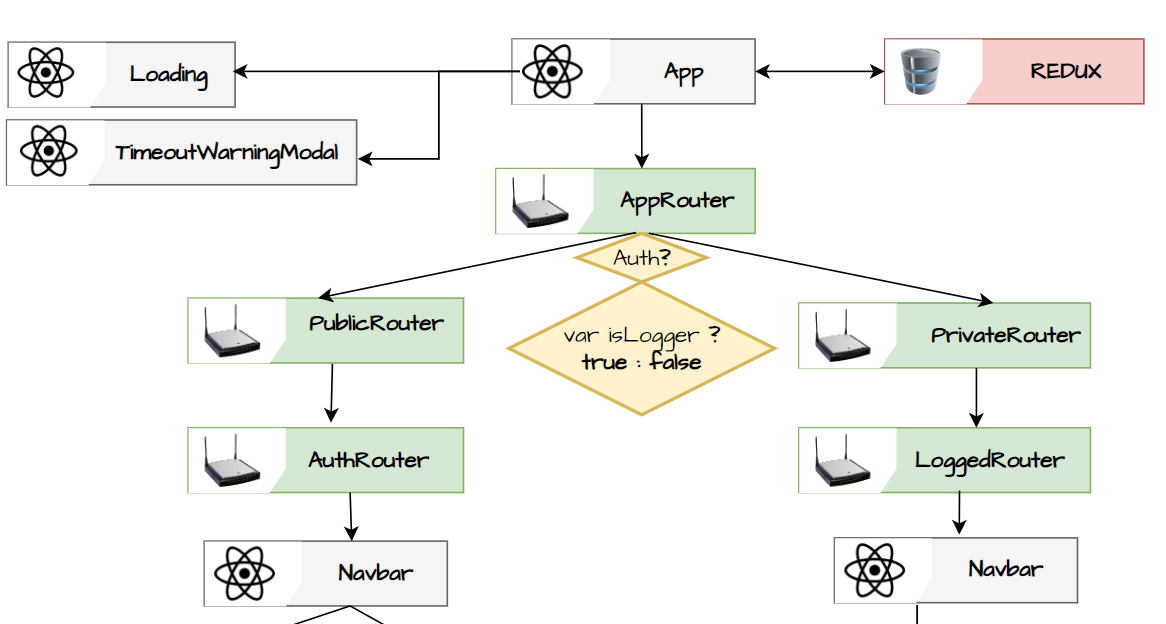
\includegraphics[width=1\linewidth]{front/front1.png}
            %\caption*{Caption}
            \label{fig:my_label}
        \end{figure}
\end{frame}
\begin{frame}{Diagrama Componentes React}
        \begin{figure}
            \centering
            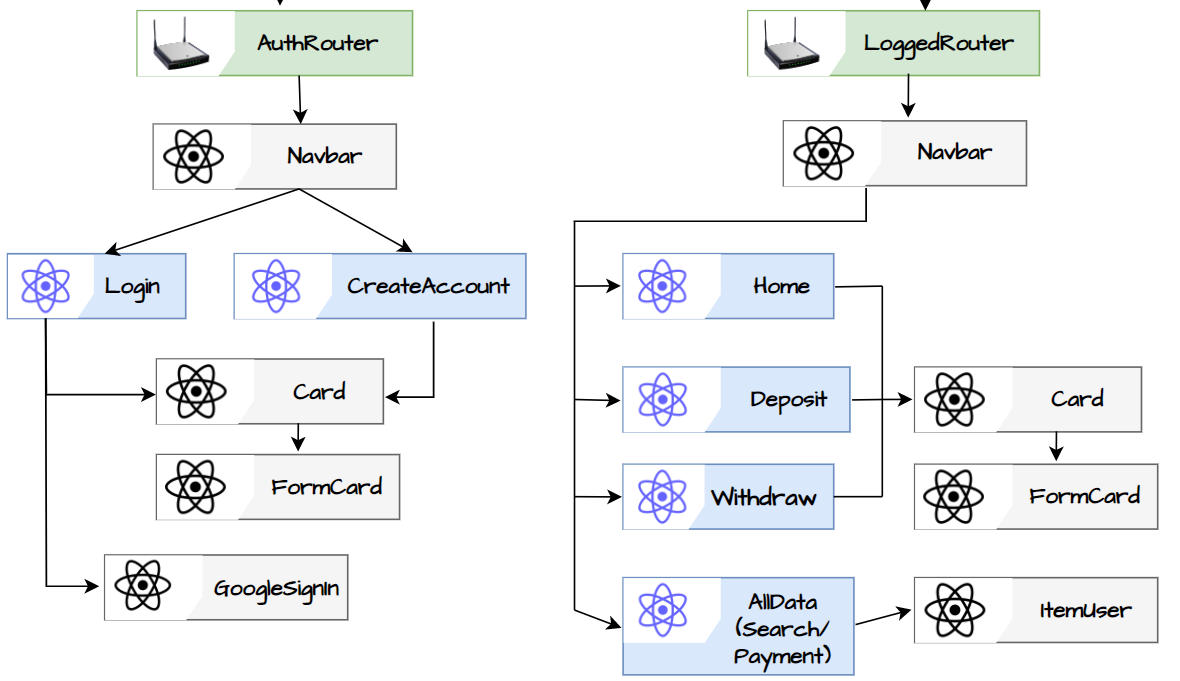
\includegraphics[width=1\linewidth]{front/front2.png}
            %\caption*{Caption}
            \label{fig:my_label}
        \end{figure}
\end{frame}
%------------------------------------------------------------
\begin{frame}{Estado de la aplicacion: Redux}
\small{
        \begin{textblock*}{0.45\textwidth}(0.05\textwidth,0.1\textwidth)
            \setbeamercolor{block title}{use=structure,fg=white,bg=violet!75!}
            \setbeamercolor{block body}{use=structure,fg=black,bg=violet!10!white}
            \begin{block}{\textbf{Redux}} 
                   Redux es un contenedor predecible del estado de aplicaciones JavaScript. Por medio de la librearia react-redux se puede utilizar en React.Caracteristicas:
                    \begin{itemize}
                        \item {Estado \textbf{global} e innmutable}
                        \item {Mayor \textbf{control} del estado de la aplicación y el flujo de datos}
                        \item {Arquitectura \textbf{escalable} de datos }
                    \end{itemize}
            \end{block}
            \vspace{-0.3cm}
            \begin{figure}
                \centering
                
\includegraphics[width=0.7\linewidth]{front/Redux.png}
                %\caption{Caption}
            \end{figure}
    \end{textblock*}
    
    \begin{textblock*}{0.45\textwidth}(0.55\textwidth,0.1\textwidth)
            \begin{figure}
                \centering
                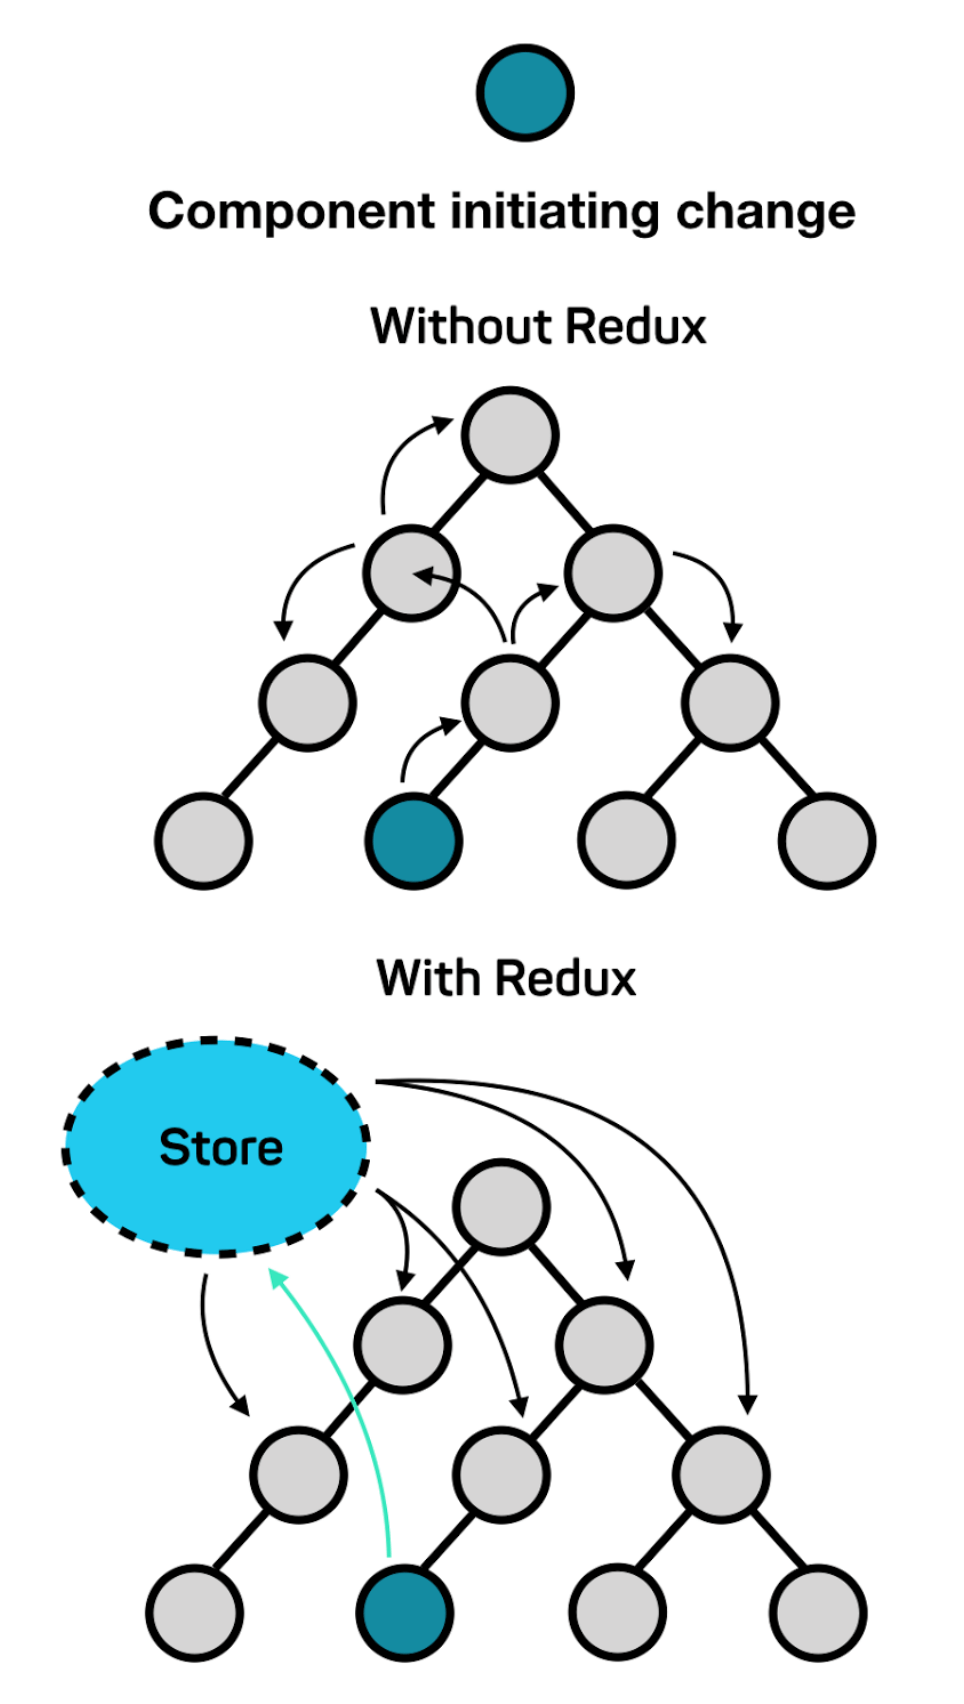
\includegraphics[width=0.8\linewidth]{front/Bildschirmfoto-2017-12-01-um-08.53.32.png}
                %\caption{Caption}
            \end{figure}
    \end{textblock*}
    

}
\end{frame}
\begin{frame}{Estado de la aplicacion: Redux}
\footnotesize {
        \begin{textblock*}{0.45\textwidth}(0.05\textwidth,0.1\textwidth)
            \setbeamercolor{block title}{use=structure,fg=white,bg=violet!75!}
            \setbeamercolor{block body}{use=structure,fg=black,bg=violet!10!white}
            \begin{block}{\textbf{Redux}} 
                    Redux en patron Flux: \textbf{Store} , \textbf{State} y \textbf{Actions + Reducers}. Los estados son:
                    \begin{itemize}
                        \item { \textbf{authUser}: Controla el estado del usuario que inicia sesión}
                        \item { \textbf{ui}: Se encarga de mostrar y ocultar componentes en situaciones particulares, como loading al hacer peticiones al servidor.}
                        \item { \textbf{allUsers}: Guarda una lista de usuarios con sus propiedades}
                    \end{itemize}
            \end{block}
            \vspace{-0.3cm}
            \begin{figure}
                \centering
                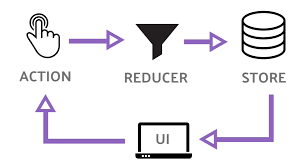
\includegraphics[width=0.8\linewidth]{front/flux.png}
                %\caption{Caption}
            \end{figure}
    \end{textblock*}
    
    \begin{textblock*}{0.45\textwidth}(0.55\textwidth,0.1\textwidth)
            \begin{figure}
                \centering
                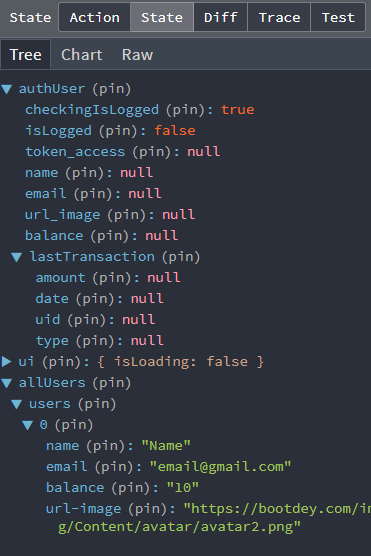
\includegraphics[width=0.87\linewidth]{front/estado redux.png}
                %\caption{Caption}
            \end{figure}
    \end{textblock*}
    

}
\end{frame}
%------------------------------------------------------------
\begin{frame}{Librerías}
        \begin{figure}
            \centering
            
\includegraphics[width=1\linewidth]{front/librerias.png}
            %\caption*{Caption}
            \label{fig:my_label}
        \end{figure}
\end{frame}
%------------------------------- [END Arquitectura Frontend ] ----------------------------------------
%------------------------------- [(3) START  Autenticacion y Autorizacion ] ----------------------------------------
\section{Autenticación}
%------------------------------------------------------------
\begin{frame}{Métodos}
\small{

    \begin{textblock*}{0.9\textwidth}(0.05\textwidth,0.1\textwidth)
        \setbeamercolor{block title}{use=structure,fg=white,bg=brown!75!}
        \setbeamercolor{block body}{use=structure,fg=black,bg=yellow!10!white}
        \begin{block}{Autenticación} 
            La autenticación es el proceso de identificar a los usuarios y garantizar que los mismos sean quienes dicen ser. Para lograr aquello en la app, se utilizan dos metodos:
                    \small {
                    \begin{itemize}
                      \setlength\itemsep{0.1em}
                        \item {\textbf{Backend Server}: Comparacion de contraseñas encriptadas en el servidor backend. Contraseñas guardadas en la base de datos. }
                        \item {\textbf{Google Verify}: Verificación por medio de un servicio externo como lo es google sign in. por medio de un token de autorización que entrega google.}
                    \end{itemize}}
            
        \end{block}
    \end{textblock*}
    
    \begin{textblock*}{0.45\textwidth}(0.05\textwidth,0.45\textwidth)
        \begin{figure}
            \centering
            
\includegraphics[width=0.45\linewidth]{auth/serverlkogo.png}
            \caption*{Backend Server}
            \label{fig:my_label}
        \end{figure}
    \end{textblock*}
    
    
    \begin{textblock*}{0.45\textwidth}(0.55\textwidth,0.45\textwidth)
        \begin{figure}
            \centering
            
\includegraphics[width=0.4\linewidth]{auth/googlelogo.png}
            \caption*{Google Sign In}
            \label{fig:my_label}
        \end{figure}
    \end{textblock*}
}
\end{frame}

%------------------------------------------------------------
\begin{frame}{Diagrama: Backend Server}
    \begin{figure}[htb]
        \centering
        \captionsetup{justification=centering,margin=0.3cm}
        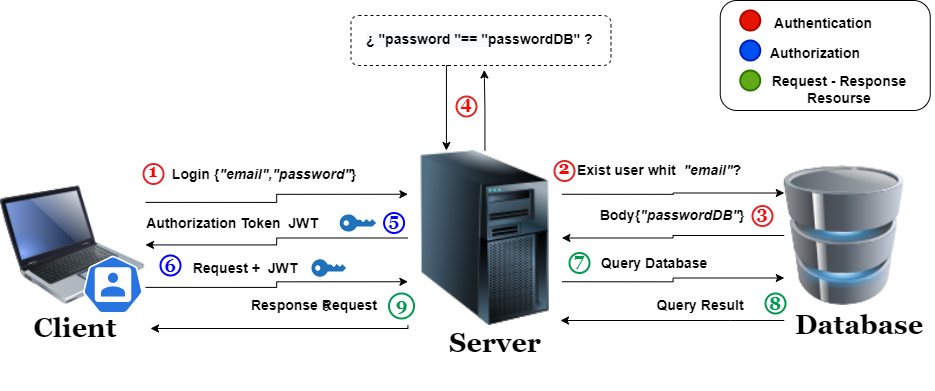
\includegraphics[width=1\linewidth]{auth/backednserer.png}
        \caption*{\footnotesize  Comparación de autenticidad con contraseña encriptada unidireccional almacenada en la base de datos. La comparacion se hace dentro del mismo servidor backend}
    \end{figure} 
\end{frame}
%------------------------------------------------------------
\begin{frame}{Diagrama: Google}
    \begin{figure}[htb]
        \centering
        \captionsetup{justification=centering,margin=0.3cm}
        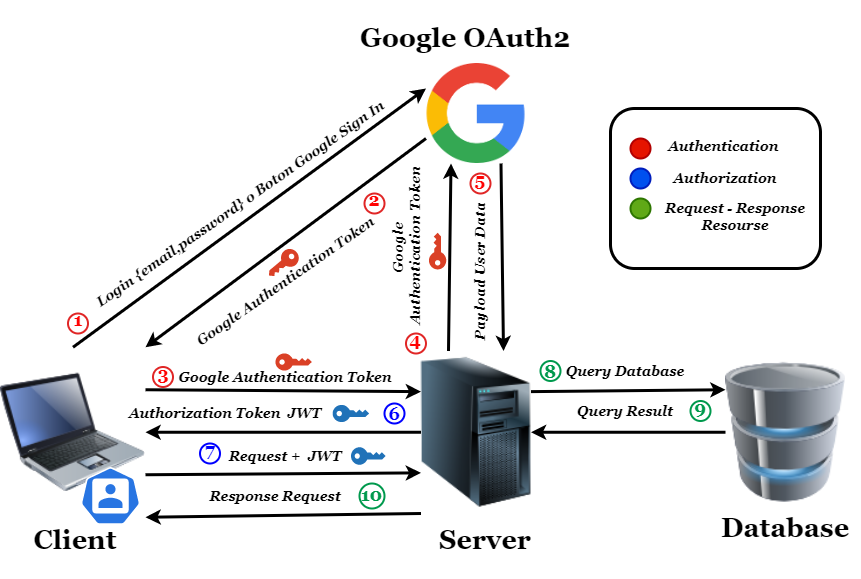
\includegraphics[width=1\linewidth]{auth/googleSignIn.png}
        \caption*{\footnotesize  Ejemplo de esquemas creados }
    \end{figure} 
\end{frame}
%------------------------------- [END  Autenticacion y Autorizacion ] ----------------------------------------

%------------------------------- [(4) START  Arquitectura Backend ] ----------------------------------------
\section{Arquitectura Backend}
%------------------------------------------------------------
\begin{frame}{Framework y Estructura de Carpetas Server}
    \begin{textblock*}{0.56\textwidth}(0.05\textwidth,0.08\textwidth)
            \setbeamercolor{block title}{use=structure,fg=white,bg=green!50!black}
            \setbeamercolor{block body}{use=structure,fg=black,bg=green!10!white}
            \begin{block}{NodeJS y Carpetas} 
            \justifying
                Se utiliza \textbf{Express} como framework de NodeJS para desarrollar el backend server de la app. La ilustracion de la derecha muestra la estructura de carpetas.
                    \vspace{-0.0cm}
                    \footnotesize {
                    \begin{itemize}
                      \setlength\itemsep{0.1em}
                        \item {\textbf{Models}: Existe una clase que configura el server y los modelos de la base datos MongoDB.}
                        \item {\textbf{Database}: Configuracion de BD Mongo Atlas y Redis.}
                        \item {\textbf{Routes}: Controla la respuesta a los endpoint segun su URI y verifica datos de entrada validos en cada peticion.}
                        \item {\textbf{Controllers}: Controla la accion a realizar para cada endpoint .}
                        \item {\textbf{Middlewares}: función que se puede ejecutar antes o después del manejo de una ruta .}
                    \end{itemize}}
            \end{block}
    \end{textblock*}
    
    
    \begin{textblock*}{0.5\textwidth}(0.6\textwidth,0.1\textwidth)
        \begin{figure}
            \centering
            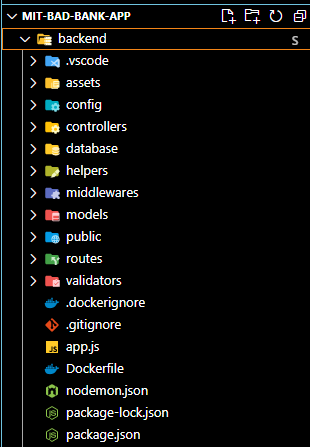
\includegraphics[width=0.75\linewidth]{back/sub.png}
            % \caption*{Espacio de trabajo robot \\ ABB irb 360-3/800}
            \label{fig:my_label}
        \end{figure}
    \end{textblock*}
\end{frame}
%------------------------------------------------------------
\begin{frame}{Base de Datos: Mongo Atlas}
    \begin{textblock*}{0.68\textwidth}(0.05\textwidth,0.1\textwidth)
            \setbeamercolor{block title}{use=structure,fg=white,bg=brown!50!black}
            \setbeamercolor{block body}{use=structure,fg=black,bg=green!5!white}
            \begin{block}{Mongo Atlas} 
            \justifying
                \textbf{MongoDB Atlas} es un servicio de \textbf{Cloud Database} (o Base de Datos en la Nube), que te permite crear y administrar tu BBDD Mongo desde cualquier lugar. Un esquema en \textbf{Mongoose }(ORM de MongoDB) es una estructura JSON que contiene información acerca de las propiedades de un documento. Se crean los siguientes esquemas:  
                    \vspace{-0.0cm}
                    \footnotesize {
                    \begin{itemize}
                      \setlength\itemsep{0.1em}
                        \item {\textbf{Users}: Usuarios registrados para realizar acciones .}
                        \item {\textbf{Roles}: Restringen que acciones pueden hacer los usuarios .}
                        \item {\textbf{Deposits}: Deposito de dinero .}
                        \item {\textbf{Whitdraws}: Retiro de dinero .}
                        \item {\textbf{StatementAccounts}: Estado de la cuenta de un usuario, como el balance de su dinero y si esta activa/bloqueada su cuenta .}
                        \item {\textbf{Payments}: Pagos entre usuarios .}
                    \end{itemize}}
            \end{block}
    \end{textblock*}
    
    
    \begin{textblock*}{0.5\textwidth}(0.65\textwidth,0.2\textwidth)
        \begin{figure}
            \centering
            
\includegraphics[width=0.7\linewidth]{bd/mongo.png}
            % \caption*{Espacio de trabajo robot \\ ABB irb 360-3/800}
            \label{fig:my_label}
        \end{figure}
    \end{textblock*}
\end{frame}
\begin{frame}{Base de Datos: Mongo Atlas}
    \begin{figure}[htb]
        \centering
        \captionsetup{justification=centering,margin=0.3cm}
        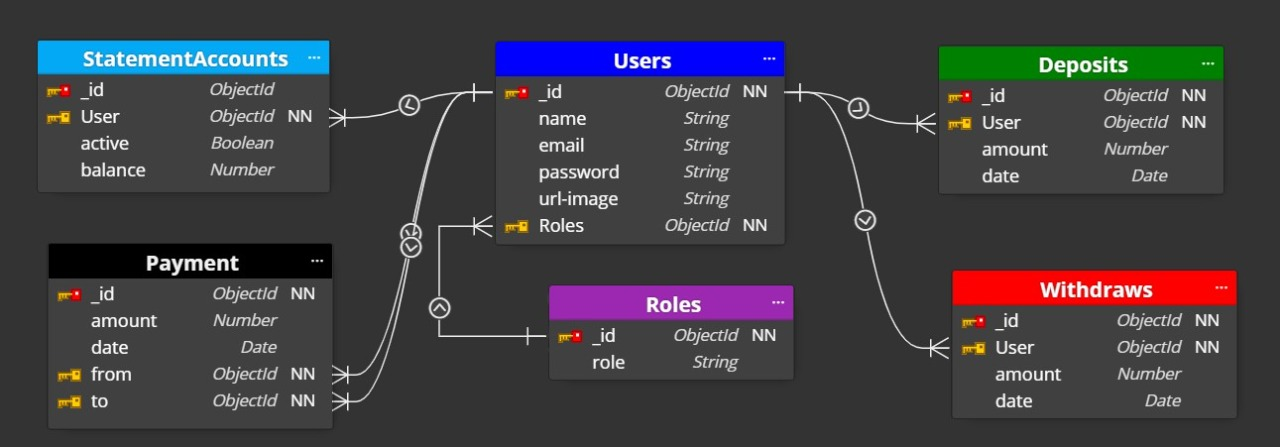
\includegraphics[width=1\linewidth]{bd/bdmongoatlas.jpeg}
        \caption*{\footnotesize  Esquemas y conexiones creados en la base de datos Mongo Atlas}
    \end{figure} 
\end{frame}
%------------------------------------------------------------

\begin{frame}{Base de Datos: Mongo Atlas}
    \begin{figure}[htb]
        \centering
        \captionsetup{justification=centering,margin=0.3cm}
        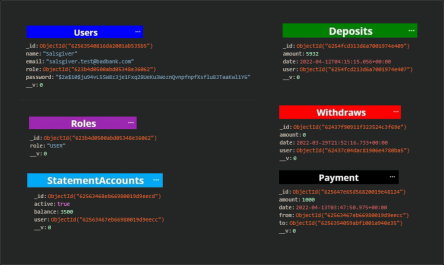
\includegraphics[width=1\linewidth]{bd/bdmiaex.png}
        \caption*{\footnotesize  Ejemplo de esquemas creados }
    \end{figure} 
\end{frame}
%------------------------------------------------------------
\begin{frame}{Base de Datos: Redis}
    \begin{textblock*}{0.55\textwidth}(0.1\textwidth,0.15\textwidth)
            \setbeamercolor{block title}{use=structure,fg=white,bg=red!50!black}
            \setbeamercolor{block body}{use=structure,fg=black,bg=red!5!white}
            \begin{block}{Redis Data Base} 
            \justifying
                \textbf{Redis}, que significa Remote Dictionary Server, es un rápido almacén de datos clave-valor en memoria de código abierto. Por medio de \textbf{Redis-Commander} se puede visualizar la base de datos. Este proyecto se utiliza Redis para guardar los token temporales de autenticación y autorización. Las clave/valor que guarda en esta app son:
                    \vspace{-0.0cm}
                    \footnotesize {
                    \begin{itemize}
                      \setlength\itemsep{0.1em}
                        \item {\textbf{Clave}: \textbf{Id} único del usuario de \textbf{MongoDB}.}
                        \item {\textbf{Valor}: JSONstringyf con un objeto que contiene \textbf{Access Token} y \textbf{Refresh Token} .}
                    \end{itemize}}
            \end{block}
    \end{textblock*}
    
    
    \begin{textblock*}{0.5\textwidth}(0.6\textwidth,0.2\textwidth)
        \begin{figure}
            \centering
            
\includegraphics[width=0.5\linewidth]{bd/red.png}
            % \caption*{Espacio de trabajo robot \\ ABB irb 360-3/800}
            \label{fig:my_label}
        \end{figure}
    \end{textblock*}
\end{frame}
%-----------------------------------------------------------
%------------------------------------------------------------
\begin{frame}{API REST: End Point}

    \begin{textblock*}{1\textwidth}(0.03\textwidth,0.05\textwidth)
        \begin{figure}
            \centering
            
\includegraphics[width=0.2\linewidth]{back/sawgger1.PNG}
            % \caption*{Espacio de trabajo robot \\ ABB irb 360-3/800}
            \label{fig:my_label}
        \end{figure}
    \end{textblock*}
    
    \begin{textblock*}{1\textwidth}(0.03\textwidth,0.12\textwidth)
        \begin{figure}
            \centering
            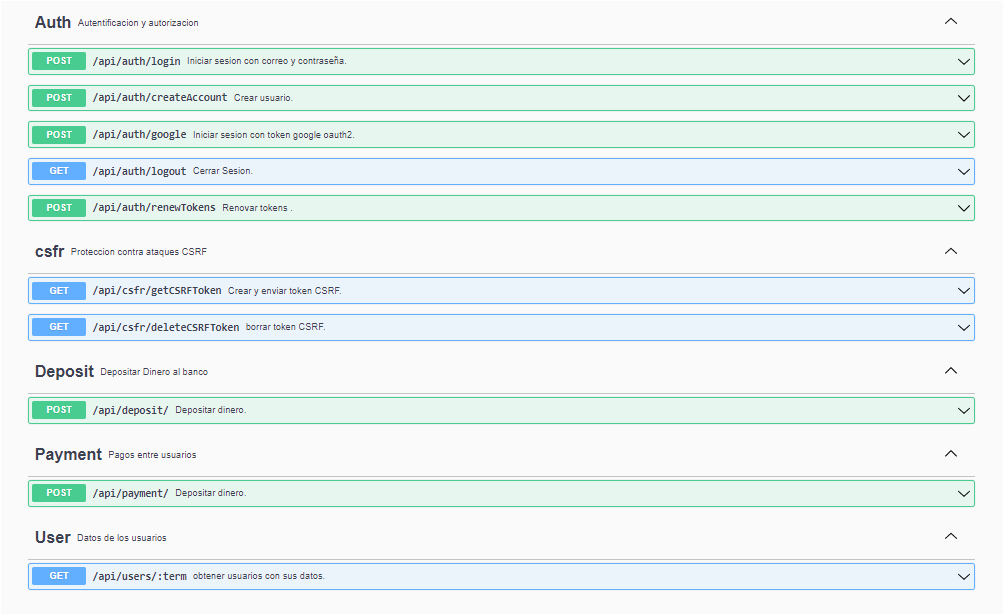
\includegraphics[width=1\linewidth]{back/sawgger2.PNG}
            % \caption*{Espacio de trabajo robot \\ ABB irb 360-3/800}
            \label{fig:my_label}
        \end{figure}
    \end{textblock*}
\end{frame}
%------------------------------- [END  Arquitectura Backend] ----------------------------------------
%------------------------------- [(5) START  Funcionalidades] ----------------------------------------
\section{Funcionalidades de la Aplicación}
%------------------------------------------------------------
\begin{frame}{Funcionalidades}
    \begin{textblock*}{0.9\textwidth}(0.1\textwidth,0.15\textwidth)
            \setbeamercolor{block title}{use=structure,fg=white,bg=red!50!black}
            \setbeamercolor{block body}{use=structure,fg=black,bg=red!5!white}
            \begin{block}{Funcionalidades} 
            \justifying
                Las principales funcionalidades de la aplicación son las siguientes acciones que puede realizar el usuario o cliente:
                    \vspace{-0.0cm}
                    \footnotesize {
                    \begin{itemize}
                      \setlength\itemsep{0.1em}
                        \item {\textbf{Crear cuenta}: con una dirección de correo electrónico y una contraseña.}
                        \item {\textbf{Inicial Sesión}: el usuario puede iniciar sesión con una dirección de correo electrónico, contraseña o autenticación OAuth 2.0 Google Sign In  .}
                        \item {\textbf{Depositar}: El usuario puede depositar dinero.}
                        \item {\textbf{Retirar}: El usuario puede retirar dinero.}
                        \item {\textbf{Base de datos}: Información del usuario y de los otros registrados en base de datos.}
                    \end{itemize}}
            \end{block}
    \end{textblock*}
    
    
    \begin{textblock*}{0.5\textwidth}(0.3\textwidth,0.57\textwidth)
        \begin{figure}
            \centering
            
\includegraphics[width=0.9\linewidth]{func/logobadbank.png}
            % \caption*{Espacio de trabajo robot \\ ABB irb 360-3/800}
            \label{fig:my_label}
        \end{figure}
    \end{textblock*}
\end{frame}
%------------------------------------------------------------
\begin{frame}{Crear cuenta: Email y Password}
    \begin{figure}[htb]
        \centering
        \captionsetup{justification=centering,margin=0.3cm}
        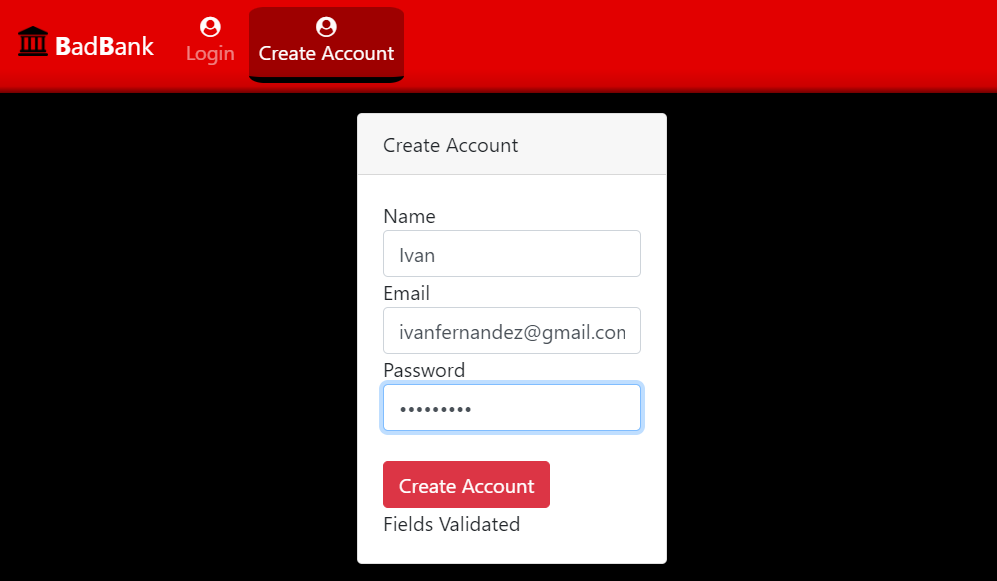
\includegraphics[width=1\linewidth]{func/cuentracrearr.png}
        % \caption*{\footnotesize  Ejemplo de esquemas creados }
    \end{figure} 
\end{frame}
%------------------------------------------------------------
\begin{frame}{Login o Crear cuenta: Google Sign In}
    \begin{figure}[htb]
        \centering
        \captionsetup{justification=centering,margin=0.3cm}
        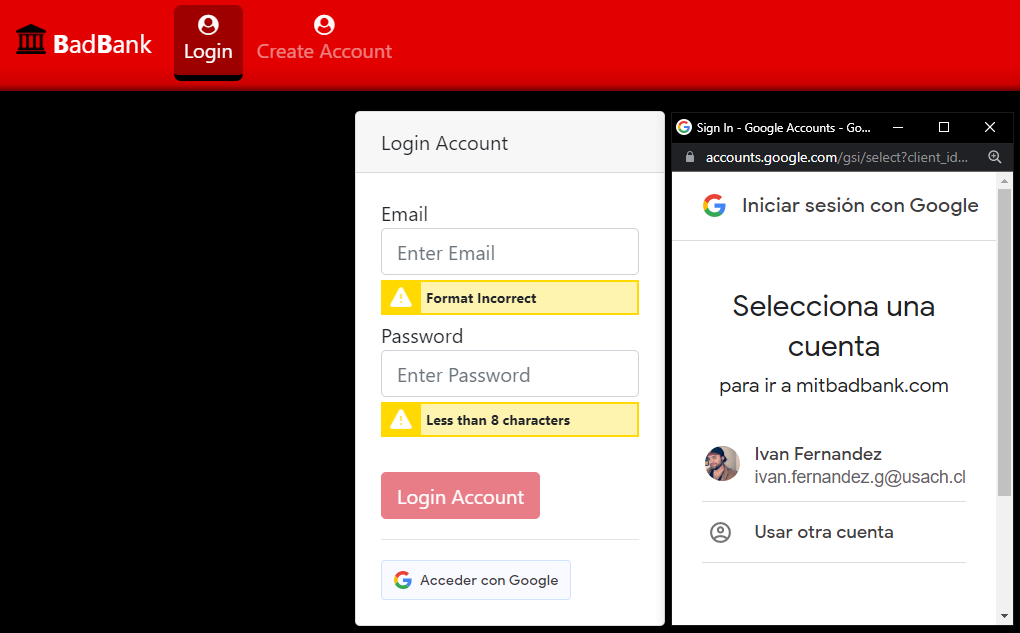
\includegraphics[width=1\linewidth]{func/Creacuentagoogle.png}
        % \caption*{\footnotesize  Ejemplo de esquemas creados }
    \end{figure}
\end{frame}
%------------------------------------------------------------
\begin{frame}{Login cuenta: Email y Password}
    \begin{figure}[htb]
        \centering
        \captionsetup{justification=centering,margin=0.3cm}
        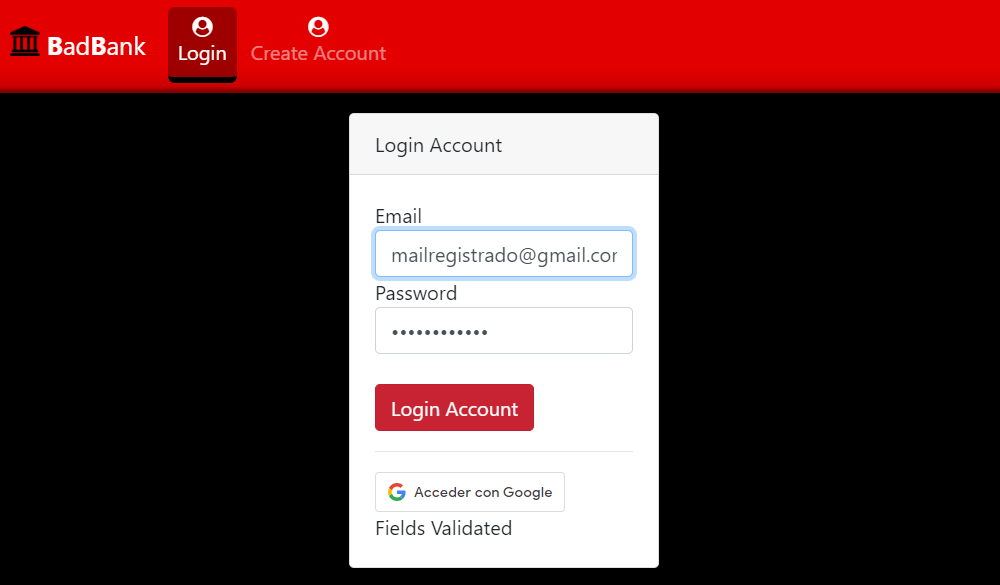
\includegraphics[width=1\linewidth]{func/LOGIN.png}
        % \caption*{\footnotesize  Ejemplo de esquemas creados }
    \end{figure}
\end{frame}

%------------------------------------------------------------
\begin{frame}{Depositar}
    \begin{figure}[htb]
        \centering
        \captionsetup{justification=centering,margin=0.3cm}
        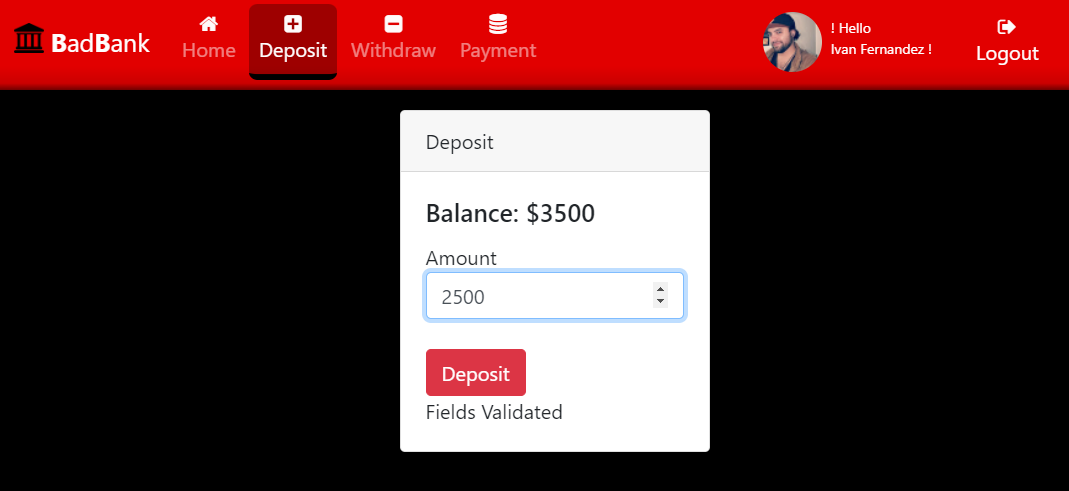
\includegraphics[width=1\linewidth]{func/depostiar.png}
        % \caption*{\footnotesize  Ejemplo de esquemas creados }
    \end{figure}
\end{frame}
%------------------------------------------------------------
\begin{frame}{Retirar}
    \begin{figure}[htb]
        \centering
        \captionsetup{justification=centering,margin=0.3cm}
        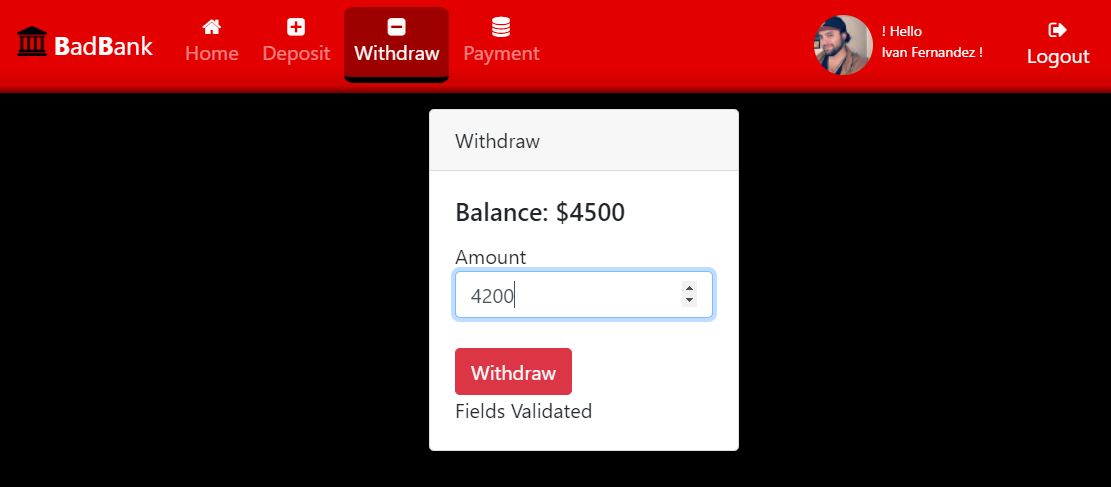
\includegraphics[width=1\linewidth]{func/retirar.png}
        % \caption*{\footnotesize  Ejemplo de esquemas creados }
    \end{figure}
\end{frame}
%------------------------------------------------------------
\begin{frame}{Persistencia base de datos Mongo Atlas}
    \begin{figure}[htb]
        \centering
        \captionsetup{justification=centering,margin=0.3cm}
        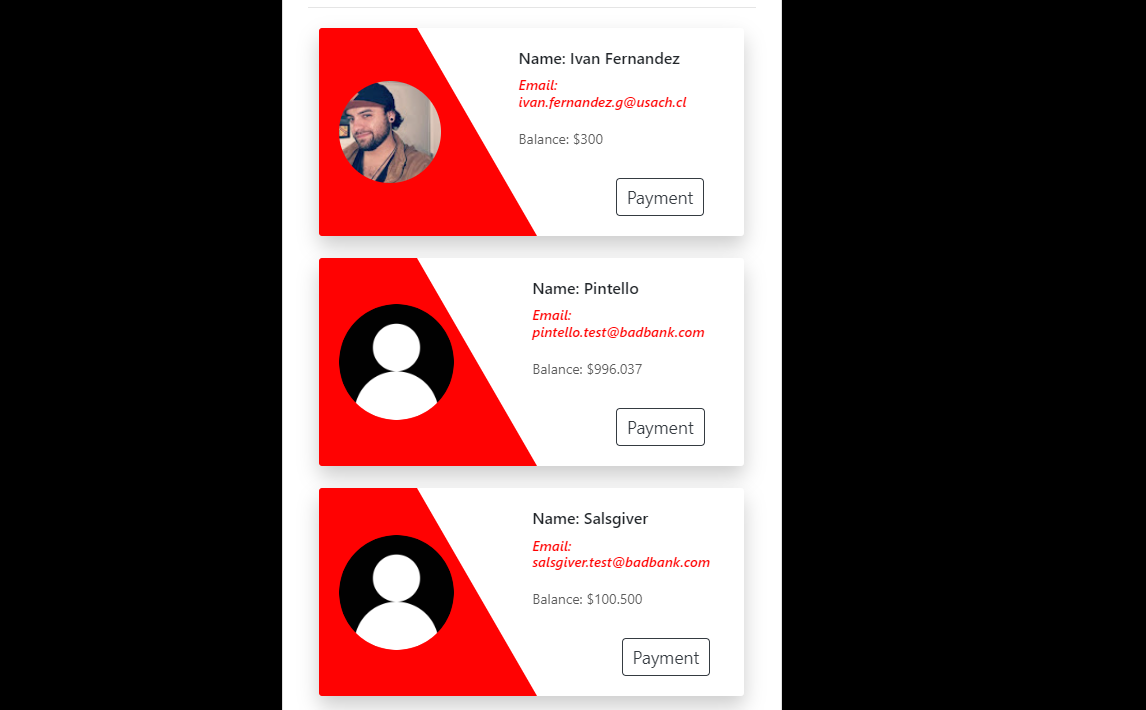
\includegraphics[width=1\linewidth]{func/representaciondedatos.png}
        % \caption*{\footnotesize  Ejemplo de esquemas creados }
    \end{figure}
\end{frame}
%------------------------------------------------------------
\begin{frame}{Persistencia base de datos Mongo Atlas}
\footnotesize {
    \begin{textblock*}{0.45\textwidth}(0.05\textwidth,0.1\textwidth)
    \begin{figure}[htb]
        \centering
        \captionsetup{justification=centering,margin=0.3cm}
        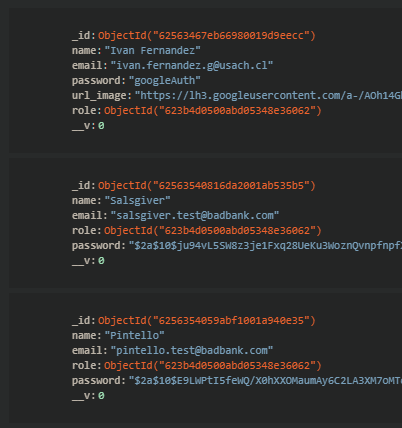
\includegraphics[width=1\linewidth]{func/basedatros.png} 
        % \caption*{\footnotesize  Ejemplo de esquemas creados }
    \end{figure}
    \end{textblock*}
    
    \begin{textblock*}{0.45\textwidth}(0.55\textwidth,0.1\textwidth)
    \begin{figure}[htb]
        \centering
        \captionsetup{justification=centering,margin=0.3cm}
        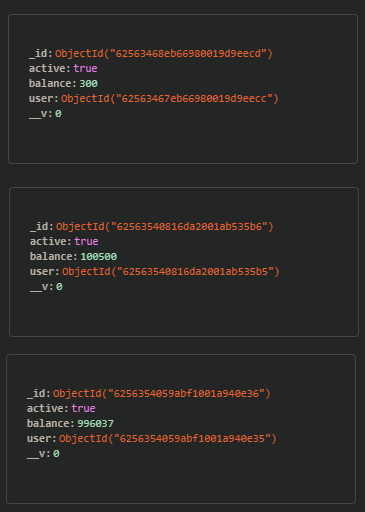
\includegraphics[width=1\linewidth]{func/stateacount .png}
        % \caption*{\footnotesize  Ejemplo de esquemas creados }
    \end{figure}
    \end{textblock*}

}


\end{frame}

%------------------------------- [END  Funcionalidades] ----------------------------------------

%------------------------------- [(6) Implementacion ] ----------------------------------------
\section{Implementacion del Proyecto}
%------------------------------------------------------------
\begin{frame}{Virtualizacion y Hosting}
\footnotesize

    \begin{textblock*}{0.48\textwidth}(0.05\textwidth,0.12\textwidth)  
            \setbeamercolor{block title}{use=structure,fg=white,bg=NavyBlue!75!black}
            \setbeamercolor{block body}{use=structure,fg=black,bg=NavyBlue!10!white}  
            \begin{block}{\textbf{Virtualizacion}} 
                                            \justifying
              \textbf{Docker} utiliza \textbf{contenedores} que incluyen todo lo necesario para que un software se ejecute. El contenedor \textbf{frontend} con Ngixn con el sitio web estatico y un balanceador de carga para las peticiones, 2 contenedores \textbf{server} con NodeJS que maneja la logica de la app y se conecta con la nube MongoDB Atlas, el contenedor \textbf{redis} para guardar tokens de seguridad y el contenedor \textbf{redis-commander} para visualizar la base de datos Redis.
            \end{block} 
    \end{textblock*}
    
    \begin{textblock*}{0.4\textwidth}(0.6\textwidth,0.12\textwidth)  
            \setbeamercolor{block title}{use=structure,fg=white,bg=orange!75!black}
            \setbeamercolor{block body}{use=structure,fg=black,bg=red!20!white}  
            \begin{block}{\textbf{Hosting}} 
                                \justifying
                \textbf{AWS Elastic Beanstalk} permite implementar, escalar servicios y aplicaciones web. EB administra de manera automática la implementación: la capacidad, el equilibrio de carga y el escalado automático hasta la monitorización del estado de la aplicación. El instancia EC2 \textbf{permite implementar contenedores docker}.
            \end{block}  
    \end{textblock*}

    \begin{textblock*}{0.48\textwidth}(0.05\textwidth,0.52\textwidth)  
                    \begin{figure}
                        \centering
                        
\includegraphics[width=0.4\linewidth]{implementacion/dockerlogo.png}
                        %\caption*{Caption}
                        \label{fig:my_label}
                    \end{figure}
    \end{textblock*}
    
    \begin{textblock*}{0.4\textwidth}(0.6\textwidth,0.5\textwidth)  
                    \begin{figure}
                        \centering
                        
\includegraphics[width=0.9\linewidth]{implementacion/eblogo.png}
                        %\caption*{Caption}
                        \label{fig:my_label}
                    \end{figure}
    \end{textblock*}
\end{frame}
%------------------------------------------------------------
\begin{frame}{Introduccion Elastic Beanstalk}
    \begin{figure}[htb]
        \centering
        \captionsetup{justification=centering,margin=0.5cm}
        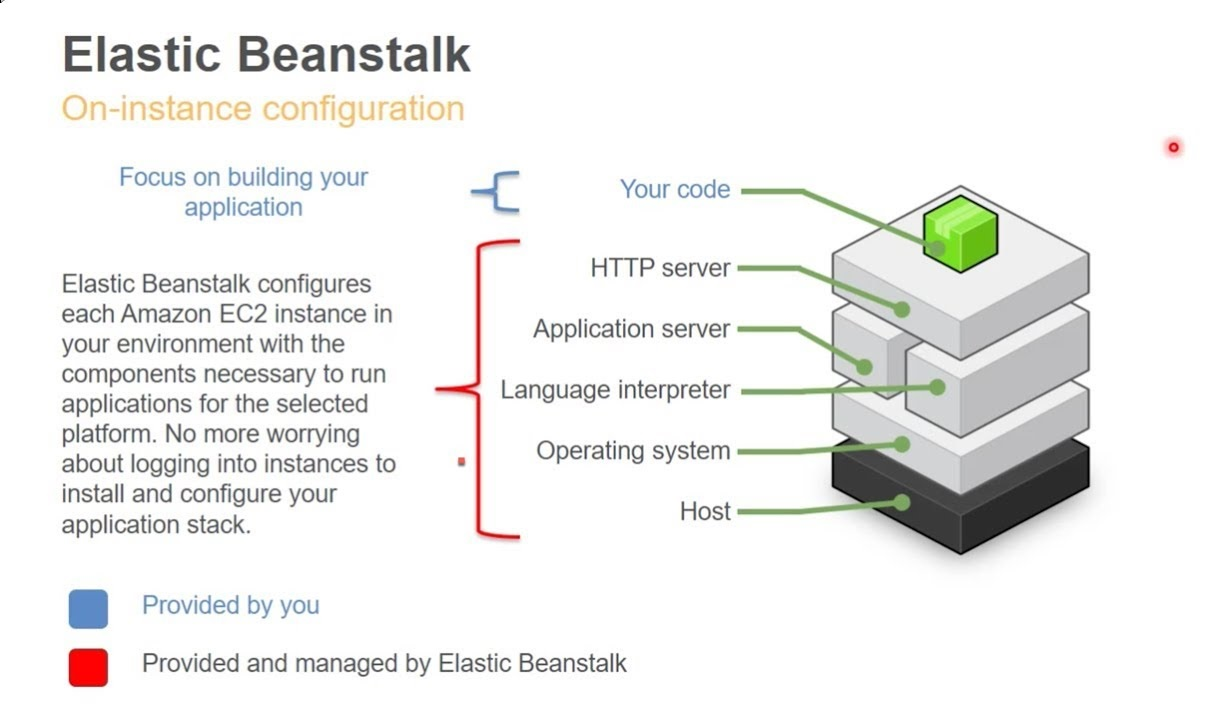
\includegraphics[width=1\linewidth]{implementacion/maxresdefault.jpg}
        % \caption*{Contenedores Docker con sus  \textbf{puertos} de escucha,  \textbf{protocolos} de peticiones,  \textbf{rutas} +  base de datos Mongodb Atlas \textbf{Cloud}}
    \end{figure}   
\end{frame}
%------------------------------------------------------------
\begin{frame}{AWS Elastic Beanstalk}
    \begin{figure}[htb]
        \centering
        \captionsetup{justification=centering,margin=0.3cm}
        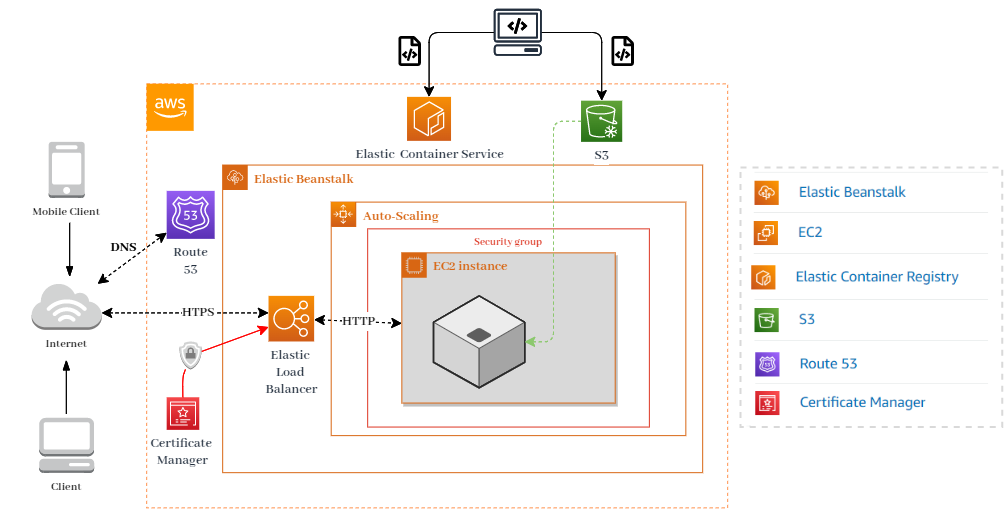
\includegraphics[width=1\linewidth]{implementacion/diagramAWS.png}
        \caption*{\footnotesize  Servicios de AWS utilizados:  \textbf{ECR} para registrar imagenes docker,  \textbf{Route3} para DNS y dominio,  \textbf{CM} para peticiones con SSl,  \textbf{ELB} para peticiones http y https,  \textbf{EC2} para la ejecucion de contenedores docker y  \textbf{S3} para almacenar los archivos(codigo) de la app en formato .zip   }
    \end{figure} 
\end{frame}
%------------------------------------------------------------
\begin{frame}{Contenedores Docker y Flujo de Peticiones}
    \begin{figure}[htb]
        \centering
        \captionsetup{justification=centering,margin=0.5cm}
        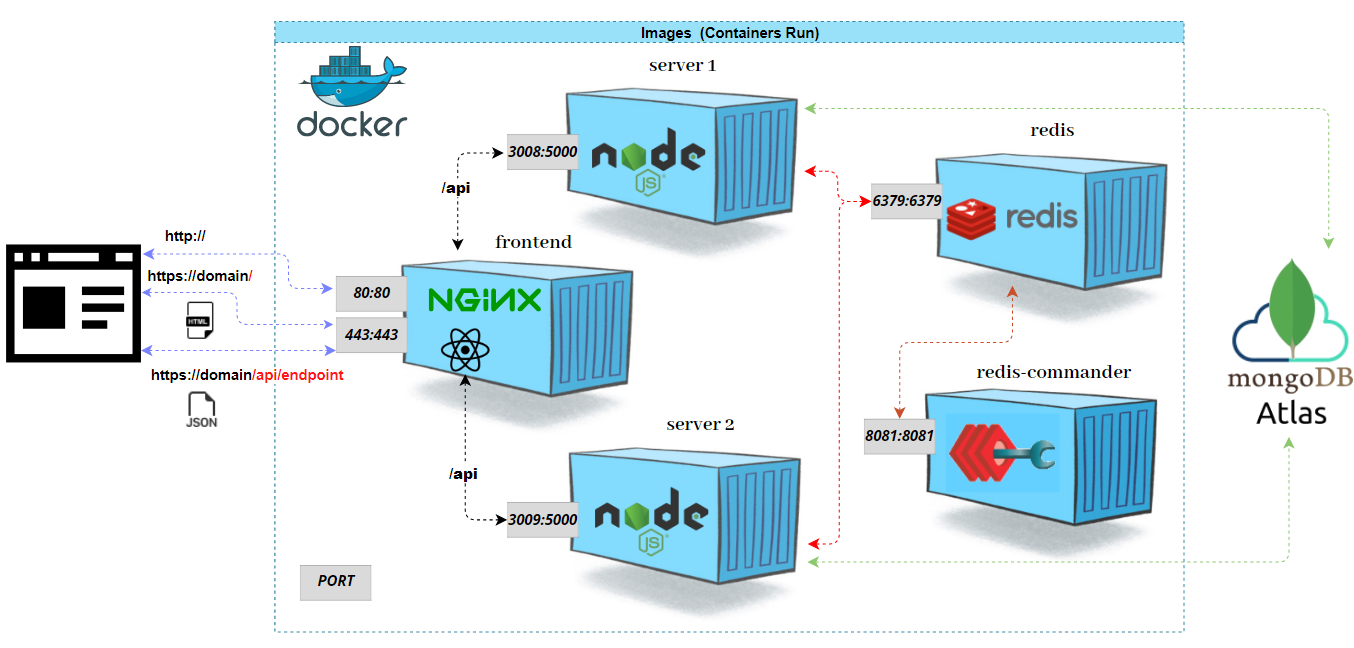
\includegraphics[width=1\linewidth]{implementacion/dockercontainers.png}
        \caption*{Contenedores Docker con sus  \textbf{puertos} de escucha,  \textbf{protocolos} de peticiones,  \textbf{rutas} +  base de datos Mongodb Atlas \textbf{Cloud}}
    \end{figure}   
\end{frame}
%------------------------------------------------------------
\begin{frame}{Docker Compose}
\footnotesize

    \begin{textblock*}{0.4\textwidth}(0.05\textwidth,0.10\textwidth)  
            \setbeamercolor{block title}{use=structure,fg=white,bg=NavyBlue!75!black}
            \setbeamercolor{block body}{use=structure,fg=black,bg=NavyBlue!10!white}  
            \begin{block}{\textbf{Multi-Contenedor}} 
                                            \justifying
                Compose es una herramienta para definir y ejecutar aplicaciones Docker de \textbf{contenedores múltiples}. Con Compose, utiliza un archivo \textbf{.YML} para configurar los servicios de su aplicación. Luego, con un solo comando, crea e inicia todos los servicios desde su configuración del archivo.
            \end{block} 
    \end{textblock*}
    
    \begin{textblock*}{0.48\textwidth}(0.52\textwidth,0.10\textwidth)  
            \setbeamercolor{block title}{use=structure,fg=white,bg=black!75!black}
            \setbeamercolor{block body}{use=structure,fg=black,bg=black!20!white}  
            \begin{block}{\textbf{Ejemplo}} 
                                \justifying
                En la ilustracion inferior se aprecia un extracto de el archivo .yml, donde se configura el contenedor \textbf{frontend} para su ejecución. Se detalla el \textbf{nombre de la imagen} y \textbf{ruta} del archivo \textbf{Dockerfile}, un archivo de \textbf{variables de entorno}, configuración de \textbf{reinicio}, \textbf{puertos} de escucha y de los \textbf{contenedores que depende}.
            \end{block}  
    \end{textblock*}

    \begin{textblock*}{0.48\textwidth}(0.05\textwidth,0.42\textwidth)  
                    \begin{figure}
                        \centering
                        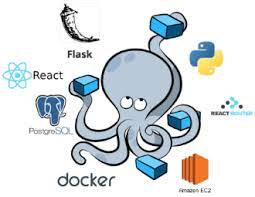
\includegraphics[width=0.8\linewidth]{implementacion/composeall.jpg}
                        %\caption*{Caption}
                        \label{fig:my_label}
                    \end{figure}
    \end{textblock*}
    
    \begin{textblock*}{0.4\textwidth}(0.6\textwidth,0.4\textwidth)  
                    \begin{figure}
                        \centering
                        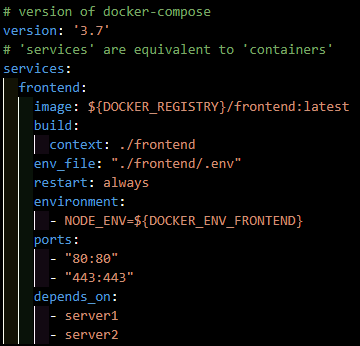
\includegraphics[width=0.9\linewidth]{implementacion/ejemplocompose.png}
                        %\caption*{Caption}
                        \label{fig:my_label}
                    \end{figure}
    \end{textblock*}
\end{frame}
%------------------------------------------------------------
\begin{frame}{Implementacion Docker + AWS EB}
        \begin{figure}
            \centering
            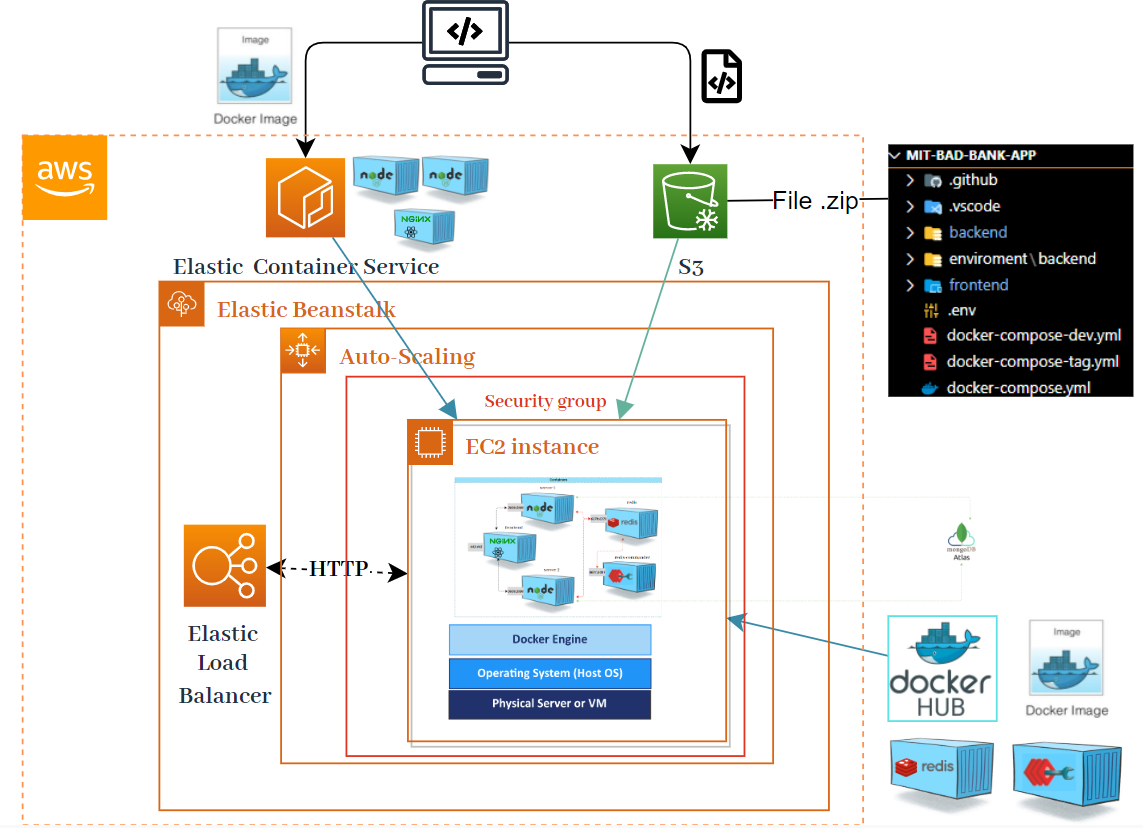
\includegraphics[width=0.9\linewidth]{implementacion/dockermasaws.png}
            %\caption*{Caption}
            \label{fig:my_label}
        \end{figure}

\end{frame}
%------------------------------- [END  Implementacion] ----------------------------------------
%------------------------------- [(7) Continous Integration & Delivery CI/CD ] ----------------------------------------
\section{Continous Integration & Delivery CI/CD}
%------------------------------------------------------------
\begin{frame}{Introduccion CI/CD}
        \begin{figure}
            \centering
            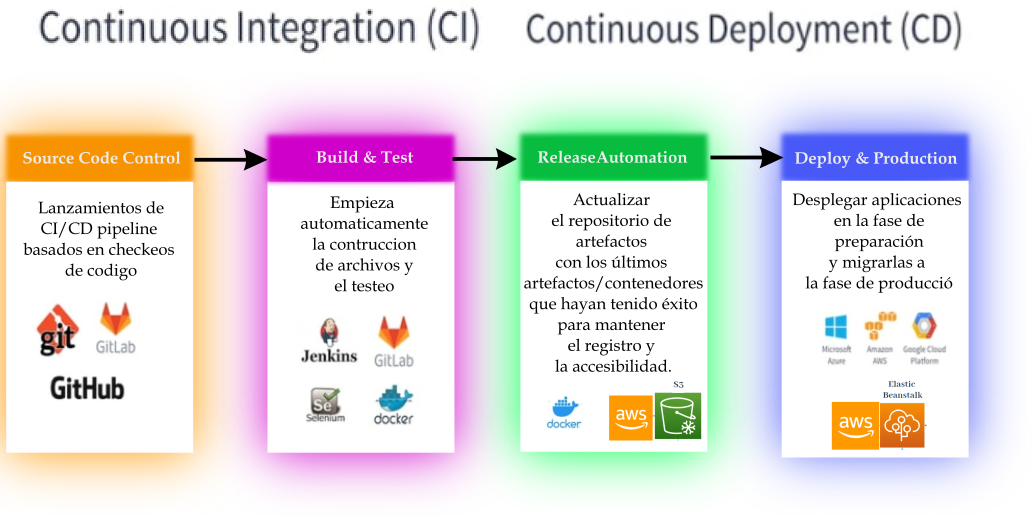
\includegraphics[width=1\linewidth]{pipeline/ejamble .png}
            %\caption*{Caption}
            \label{fig:my_label}
        \end{figure}
\end{frame}
%------------------------------------------------------------
\begin{frame}{Resumen pipeline}

\setbeamercolor{block title}{use=structure,fg=white,bg=Limegreen!75!}
\setbeamercolor{block body}{use=structure,fg=black,bg=Limegreen!10!white}
\begin{block}{Workflow de la aplicacion}
    \justifying
    \begin{itemize}
    \item {El desarollador aloja en \textbf{repositorios en github} los codigos de la app con el sistema de \textbf{versiones git}. En cada nueva version del codigo alojado, github \textbf{activa una accion}, la cual tiene el fin de \textbf{subir a produccion la app a AWS}.}
    \end{itemize}
\end{block}

\begin{figure}
        \centering
        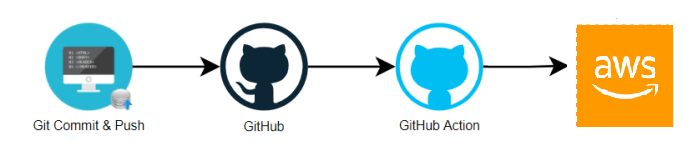
\includegraphics[width=0.9\linewidth]{pipeline/basicdeploy.png}
        %\caption*{Caption}
        \label{fig:my_label}
    \end{figure}
\end{frame}
%------------------------------------------------------------
\begin{frame}{Workflow & Pipeline}
        \begin{figure}
            \centering
            \includegraphics[width=1\linewidth]{pipeline/pipeline2.png}
            %\caption*{Caption}
            \label{fig:my_label}
        \end{figure}
\end{frame}

%------------------------------- [END  Continous Integration & Delivery CI/CD ] ----------------------------------------
%------------------------------- [(8) Extras ] ----------------------------------------
\section{Extras: Cyber Security, UI, Roles}
%------------------------------------------------------------
\begin{frame}{Cyber Security: AccessToken y Refresh Token }
    \scriptsize {
    \begin{textblock*}{0.95\textwidth}(0.05\textwidth,0.08\textwidth)
            \setbeamercolor{block title}{use=structure,fg=white,bg=red!50!black}
            \setbeamercolor{block body}{use=structure,fg=black,bg=red!5!white}
            \begin{block}{Autorizacion y Seguridad} 
            \justifying
                Con el fin de \textbf{proteger los datos} para que no sean enviados a personas no autorizadas, se crear 2 tokens. Estos se entregan después de la \textbf{autenticación} (iniciar sesión). Un  \textbf{midleware} en el server verifica en cada peticion que necesite autorizacion si estos tokens son validos
                    \vspace{-0.04cm}
                    \scriptsize{
                    \begin{itemize}
                      \setlength\itemsep{0.1em}
                        \item {\textbf{Access Token}: Utilizado como  \textbf{permiso para pedir recursos a la API}. Contiene id del usuario y expira rápidamente. Se guarda en  \textbf{memoria}, es decir, en una estado o \textbf{variable JS}.}
                        \item {\textbf{Refresh Token}: Se utiliza para  \textbf{validar la creación de un Access Token} cuando este ultimo expira. Contiene id del usuario y tiene un tiempo de expiración mayor al Access token. Para evitar ataques de hackers  \textbf{cross-site scripting(XSS)} se guarda en una  \textbf{cookie.} }
                    \end{itemize}}
            \end{block}
    \end{textblock*}}
    
    
    \begin{textblock*}{1\textwidth}(0.03\textwidth,0.37\textwidth)
        \begin{figure}
            \centering
            \includegraphics[width=1\linewidth]{cyber/2SEGURITY.png}
            % \caption*{Espacio de trabajo robot \\ ABB irb 360-3/800}
            \label{fig:my_label}
        \end{figure}
    \end{textblock*}
\end{frame}
%------------------------------------------------------------
\begin{frame}{Cyber Security: AccessToken y Refresh Token }
\footnotesize

    \begin{textblock*}{0.64\textwidth}(0.05\textwidth,0.10\textwidth)  
                    \begin{figure}
                        \centering
                        \includegraphics[width=1\linewidth]{cyber/3SEGURITY1.png}
                        \caption*{Refresh Token guardado en navegador como una cookie (Frontend)}
                        \label{fig:my_label}
                    \end{figure}
    \end{textblock*}
    

    \begin{textblock*}{0.3\textwidth}(0.7\textwidth,0.18\textwidth)  
                    \begin{figure}
                        \centering
                        \includegraphics[width=1\linewidth]{cyber/3SEGURITY2REDUX.png}
                        \caption*{Access Token guardado en estado Redux en React (Frontend)}
                        \label{fig:my_label}
                    \end{figure}
    \end{textblock*}

    \begin{textblock*}{0.64\textwidth}(0.05\textwidth,0.33\textwidth)  
                    \begin{figure}
                        \centering
                        \includegraphics[width=1\linewidth]{cyber/3SEGURITY3REdis.png}
                        \caption*{Access y Refresh Token guardado en Redis para verificaciones de autorización en el server (backend)}
                        \label{fig:my_label}
                    \end{figure}
    \end{textblock*}
    \end{frame}
%------------------------------------------------------------
\begin{frame}{Cyber Security: AccessToken y Refresh Token }
        \begin{figure}
            \centering
            \includegraphics[width=1\linewidth]{cyber/4SEGURITY.pngexpiracion.png}
            \caption*{ Estado para realizar peticiones a la API, renovación de tokens, tiempo de expiración de tokens y logout. }
            \label{fig:my_label}
        \end{figure}\end{frame}
%------------------------------------------------------------
\begin{frame}{Cyber Security: Middleware verificacion Tokens }
        \begin{figure}
            \centering
            \includegraphics[width=0.7\linewidth]{cyber/5diagrama1.PNG}
            %\caption*{Caption}
            \label{fig:my_label}
        \end{figure}
\end{frame}
%------------------------------------------------------------
\begin{frame}{Cyber Security: Middleware verificacion Tokens }
        \begin{figure}
            \centering
            \includegraphics[width=0.9\linewidth]{cyber/5diagrama2.PNG}
            %\caption*{Caption}
            \label{fig:my_label}
        \end{figure}
\end{frame}
%------------------------------------------------------------
\begin{frame}{Cyber Security: Middleware verificacion Tokens }
        \begin{figure}
            \centering
            \includegraphics[width=0.9\linewidth]{cyber/5diagrama3.PNG}
            %\caption*{Caption}
            \label{fig:my_label}
        \end{figure}
\end{frame}
%------------------------------------------------------------
\begin{frame}{Cyber Security:  Autenticación y Autorización  }
        \begin{figure}
            \centering
            \includegraphics[width=1\linewidth]{cyber/6SEGURITYFINALGOOGLE .png}
            %\caption*{Caption}
            \label{fig:my_label}
        \end{figure}
\end{frame}
%------------------------------------------------------------
\begin{frame}{Cyber Security: CSRF Token}
    \scriptsize{
    \begin{textblock*}{0.95\textwidth}(0.05\textwidth,0.1\textwidth)
            \setbeamercolor{block title}{use=structure,fg=white,bg=violet!50!black}
            \setbeamercolor{block body}{use=structure,fg=black,bg=violet!5!white}
            \begin{block}{Autorizacion y Seguridad} 
            \justifying
               Con el fin de proteger los datos de un ataque \textbf{Cross Site Request Forgery (CSRF)} se crean 2 token. Uno es enviado en el  \textbf{body} de una respuesta a un endpoint especifico para pedir estos tokens y se guarda en un \textbf{tag en html} (recomendable dentro de <head>). El otro se envia por medio de una  \textbf{cookie}. El  \textbf{tiempo de expiracion} de este token es 2 veces el Refresh Token (120 [s]). Un  \textbf{midleware} en el server verifica que estos dos token tengan una relación valida cada vez que se envía una petición distinta a GET.
                    \vspace{-0.04cm}
            \end{block}
    \end{textblock*}}
    
    
    \begin{textblock*}{1\textwidth}(0.03\textwidth,0.327\textwidth)
        \begin{figure}
            \centering
            \includegraphics[width=1\linewidth]{cyber/CSRFFLUJO.png}
            % \caption*{Espacio de trabajo robot \\ ABB irb 360-3/800}
            \label{fig:my_label}
        \end{figure}
    \end{textblock*}
\end{frame}
%------------------------------------------------------------
\begin{frame}{Cyber Security: CSRF Token}
        \begin{figure}
            \centering
            \includegraphics[width=1\linewidth]{cyber/csfr.PNG} 
            \caption*{Token guardado en tag html}
            \label{fig:my_label}
        \end{figure}
        
        \begin{figure}
            \centering
            \includegraphics[width=1\linewidth]{cyber/cockie csrf y refresh.PNG} 
            \caption*{Token guardado den una cookie}
            \label{fig:my_label}
        \end{figure}
\end{frame}
%------------------------------------------------------------
\begin{frame}{CS: Autenticacion, Autorizacion y CSRF}
        \begin{figure}
            \centering
            \includegraphics[width=1\linewidth]{cyber/TOFDO.png}
            %\caption*{Caption}
            \label{fig:my_label}
        \end{figure}
\end{frame}
%------------------------------------------------------------
\begin{frame}{Payment}
    \begin{figure}[htb]
        \centering
        \captionsetup{justification=centering,margin=0.3cm}
        \includegraphics[width=0.9\linewidth]{extras/payemn1.png}
        % \caption*{\footnotesize  Servicios de AWS utilizados:  \textbf{pa} para   }
    \end{figure} 
\end{frame}
%------------------------------------------------------------
\begin{frame}{Timeout Session}
    \begin{figure}[htb]
        \centering
        \captionsetup{justification=centering,margin=0.3cm}
        \includegraphics[width=0.9\linewidth]{extras/timessesion.png}
        \caption*{\footnotesize Modal que avisa que  el \textbf{Refresh Token} pronto expirara }. Si quieres seguir en la sesión, debes pedir nuevos \textbf{Refresh Token y Access Token} haciendo click en el boton verde. Esta función también pide un nuevo token CSRF. 
    \end{figure} 
\end{frame}
%------------------------------------------------------------
\begin{frame}{Search Users}
    \begin{figure}[htb]
        \centering
        \captionsetup{justification=centering,margin=0.3cm}
        \includegraphics[width=0.8\linewidth]{extras/serch.png}
        % \caption*{\footnotesize  Servicios de AWS utilizados:  \textbf{ECR} para   }
    \end{figure} 
\end{frame}
%------------------------------------------------------------
\begin{frame}{Loading}
    \begin{figure}[htb]
        \centering
        \captionsetup{justification=centering,margin=0.3cm}
        \includegraphics[width=0.5\linewidth]{extras/LOADIN.png}
        \caption*{\footnotesize  Animación en la interfaz cuando se realizan  \textbf{peticiones fetch al servidor}. Son tres círculos rojos girando sobre su eje central y crea un estilo de fondo blanco con opacidad }
    \end{figure} 
\end{frame}
%------------------------------------------------------------
\begin{frame}{Logout}
    \begin{figure}[htb]
        \centering
        \captionsetup{justification=centering,margin=0.3cm}
        \includegraphics[width=0.8\linewidth]{extras/logout.png}
        \caption*{\footnotesize  La funcion logout hace una peticion al servidor para  \textbf{eliminar el Access Token y Refresh Token} de la base de datos Redis y manda una respuesta eliminando el Refresh token del navegador.   }
    \end{figure} 
\end{frame}
%------------------------------------------------------------
\begin{frame}{Roles Backend Server}
    \begin{figure}[htb]
        \centering
        \captionsetup{justification=centering,margin=0.3cm}
        \includegraphics[width=0.6\linewidth]{extras/roles.png}
        \caption*{\footnotesize{  \textbf{3 Roles} ("DBADMIN", "DEV", "USER") ingresados manualmente por seguridad a base de datos Mongo Atlas por medio de Mongo Compass. Estos roles son para  \textbf{restringir los endpoint} a ciertos usuarios. Esto se implementa por medio de un middleware en los router de el server backend}}
    \end{figure} 
\end{frame}
%------------------------------- [END  Extras] ----------------------------------------

%------------------------------- [(9) Referencias ] ----------------------------------------
\section{Referencias}
%------------------------------------------------------------
\begin{frame}{Referencias}
    \begin{textblock*}{0.7\textwidth}(0.1\textwidth,0.2\textwidth)  
        \justifying
        \small
        \setbeamercolor{block title}{use=structure,fg=white,bg=red!75!black}
        \setbeamercolor{block body}{use=structure,fg=black,bg=red!10!white}		
        \begin{block}{URL de la pagina web}
            \justifying
            https://mitbadbank.com/ 
        \end{block}	
        
                \setbeamercolor{block title}{use=structure,fg=white,bg=black!75!black}
        \setbeamercolor{block body}{use=structure,fg=black,bg=black!10!white}		
        \begin{block}{URL del Repositorio Github}
            \justifying
            https://github.com/IvanFernandezGracia/MIT-BadBankApp
        \end{block}	

                \setbeamercolor{block title}{use=structure,fg=white,bg=blue!75!black}
        \setbeamercolor{block body}{use=structure,fg=black,bg=blue!10!white}		
        \begin{block}{Linkedin}
            \justifying
            https://www.linkedin.com/in/ivan-fg/
        \end{block}	
        
    \end{textblock*}
\end{frame}
%------------------------------- [END  Referencias] ----------------------------------------




%%%%%%%%%%%%%%%%%%%%%%%%%%%%%%%%%%%%%%%%%%%%%%%%%%%%%%%%%%%%%%%%%%%%%%%%%%%%%%%%%%%%%%%%%%%%%%%%%%%%%%%%%%%%%%%%%%%%%%%%%%%%%%%%%%%%%%%%%%%%%%%%%%%%%%%%%%%%%%%%%%%%%%%%%%%%%%%%%%%%%%%%%%%%%%%%%%%%%%%%%%%%%%%%%%%%%%%%%%%%%%%%%%%%%%%%%%%%%%%%%%%%%%%%%%%%%%%%%%%%%%%%%%%%%%%%%%%%%%%%%%%%%%%%%%%%%%%%%%%%%%%%%%%%%%%%%%%%%%%%%%%%%%%%%%%%%%%%%%%%%%%%%%%%%%%%%%%%%%%%%%%%%%%%%%%%%%%%%%%%%%%%%%%%%%%%%%%%%%%%%%%%%%%%%%%%%%%%%%%%%%%%%%%%%%%%%%%%%%%%%%%%%%%%%%%%%%%%%%%%%%%%%%%%%%%%%%%%%%%%%%%%%%%%%%%%%%%%%%%%%%%%%%%%%%%%%%%%%%%%%%%%%%%%%%%%%%%%%%%%%%%%%%%%%%%%%%%%%%%%%%%%%%%%%%%%%%%%%%%%%%%%%%%%%%%%%%%%%%%%%%%%%%%%%%%%%%%%%%%%%%%%%%%%%%%%%%%%%%%%%%%%%%%%%%%%%%%%%%%%%%%%%%%%%%%%%%%%%%%%%%%%%%%%%%%%%%%%%%%%%%%%%%%%%%%%%%%%%%%%%%%%%%%%%%%%%%%%%%%%%%%%%%%%%%%%%%%%%%%%%%%%%%%%%%%%%%%%%%%%%%%%%%%%%%%%%%%%%%%%%%%%%%%%%%%%%%%%%%%%%%%%%%%%%%%%%%%%%%%%%%%%%%%%%%%%%%%%%%%%%%%%%%%%%%%%%%%%%%%%%%%%%%%%%%%%%%%%%%%%%%%%%%%%%%%%%%%%%%%%%%%%%%%%%%%%%%%%%%%%%%%%%%%%%


\end{document}
